\documentclass[a4paper, 12pt]{book}
%\documentclass[a4paper, 12pt, draft]{book}  Nalogo preverite tudi z opcijo draft, ki vam bo pokazala, katere vrstice so predolge!

\usepackage[utf8x]{inputenc}   % omogoča uporabo slovenskih črk kodiranih v formatu UTF-8
\usepackage[slovene,english]{babel}    % naloži, med drugim, slovenske delilne vzorce
\usepackage[pdftex]{graphicx}  % omogoča vlaganje slik različnih formatov
\usepackage{fancyhdr}          % poskrbi, na primer, za glave strani
\usepackage{amssymb}           % dodatni simboli
\usepackage{amsmath}           % eqref, npr.
%\usepackage{hyperxmp}
\usepackage[hyphens]{url}  % dodal Solina
\usepackage{comment}       % dodal Solina

\usepackage[pdftex, colorlinks=true,
                        citecolor=black, filecolor=black, 
                        linkcolor=black, urlcolor=black,
                        pagebackref=false, 
                        pdfproducer={LaTeX}, pdfcreator={LaTeX}, hidelinks]{hyperref}

\usepackage{color}       % dodal Solina
\usepackage{soul}       % dodal Solina

\usepackage{longtable}  % dodal jaz
\usepackage{makecell}   % dodal jaz
\usepackage{minted}     % dodal jaz
\usemintedstyle{bw}     % dodal jaz

%%%%%%%%%%%%%%%%%%%%%%%%%%%%%%%%%%%%%%%%
%	DIPLOMA INFO
%%%%%%%%%%%%%%%%%%%%%%%%%%%%%%%%%%%%%%%%
\newcommand{\ttitle}{Visoko skalabilna NewSQL relacijska podatkovna baza CockroachDB}
\newcommand{\ttitleEn}{Higly Scalable NewSQL Relational Database CockroachDB}
\newcommand{\tsubject}{\ttitle}
\newcommand{\tsubjectEn}{\ttitleEn}
\newcommand{\tauthor}{Matjaž Mav}
\newcommand{\tkeywords}{podatkovne baze, skaliranje, SQL, NewSQL, CockroachDB, PostgreSQL, Citus, YCSB}
\newcommand{\tkeywordsEn}{databases, scalability, SQL, NewSQL, PostgreSQL, Citus, YCSB}


%%%%%%%%%%%%%%%%%%%%%%%%%%%%%%%%%%%%%%%%
%	HYPERREF SETUP
%%%%%%%%%%%%%%%%%%%%%%%%%%%%%%%%%%%%%%%%
\hypersetup{pdftitle={\ttitle}}
\hypersetup{pdfsubject=\ttitleEn}
\hypersetup{pdfauthor={\tauthor, mm3058@student.uni-lj.si}}
\hypersetup{pdfkeywords=\tkeywordsEn}


    


%%%%%%%%%%%%%%%%%%%%%%%%%%%%%%%%%%%%%%%%
% postavitev strani
%%%%%%%%%%%%%%%%%%%%%%%%%%%%%%%%%%%%%%%%  

\addtolength{\marginparwidth}{-20pt} % robovi za tisk
\addtolength{\oddsidemargin}{40pt}
\addtolength{\evensidemargin}{-40pt}

\renewcommand{\baselinestretch}{1.3} % ustrezen razmik med vrsticami
\setlength{\headheight}{15pt}        % potreben prostor na vrhu
\renewcommand{\chaptermark}[1]%
{\markboth{\MakeUppercase{\thechapter.\ #1}}{}} \renewcommand{\sectionmark}[1]%
{\markright{\MakeUppercase{\thesection.\ #1}}} \renewcommand{\headrulewidth}{0.5pt} \renewcommand{\footrulewidth}{0pt}
\fancyhf{}
\fancyhead[LE,RO]{\sl \thepage} 
%\fancyhead[LO]{\sl \rightmark} \fancyhead[RE]{\sl \leftmark}
\fancyhead[RE]{\sc \tauthor}              % dodal Solina
\fancyhead[LO]{\sc Diplomska naloga}     % dodal Solina


\newcommand{\BibTeX}{{\sc Bib}\TeX}

%%%%%%%%%%%%%%%%%%%%%%%%%%%%%%%%%%%%%%%%
% naslovi
%%%%%%%%%%%%%%%%%%%%%%%%%%%%%%%%%%%%%%%%  


\newcommand{\autfont}{\Large}
\newcommand{\titfont}{\LARGE\bf}
\newcommand{\clearemptydoublepage}{\newpage{\pagestyle{empty}\cleardoublepage}}
\setcounter{tocdepth}{2}	      % globina kazala

%%%%%%%%%%%%%%%%%%%%%%%%%%%%%%%%%%%%%%%%
% konstrukti
%%%%%%%%%%%%%%%%%%%%%%%%%%%%%%%%%%%%%%%%  
\newtheorem{izrek}{Izrek}[chapter]
\newtheorem{trditev}{Trditev}[izrek]
\newenvironment{dokaz}{\emph{Dokaz.}\ }{\hspace{\fill}{$\Box$}}

%%%%%%%%%%%%%%%%%%%%%%%%%%%%%%%%%%%%%%%%%%%%%%%%%%%%%%%%%%%%%%%%%%%%%%%%%%%%%%%
%% PDF-A
%%%%%%%%%%%%%%%%%%%%%%%%%%%%%%%%%%%%%%%%%%%%%%%%%%%%%%%%%%%%%%%%%%%%%%%%%%%%%%%


%%%%%%%%%%%%%%%%%%%%%%%%%%%%%%%%%%%%%%%% 
% define medatata
%%%%%%%%%%%%%%%%%%%%%%%%%%%%%%%%%%%%%%%% 
\def\Title{\ttitle}
\def\Author{\tauthor, mm3058@student.uni-lj.si}
\def\Subject{\ttitleEn}
\def\Keywords{\tkeywordsEn}

%%%%%%%%%%%%%%%%%%%%%%%%%%%%%%%%%%%%%%%% 
% \convertDate converts D:20080419103507+02'00' to 2008-04-19T10:35:07+02:00
%%%%%%%%%%%%%%%%%%%%%%%%%%%%%%%%%%%%%%%% 
\def\convertDate{%
    \getYear
}

{\catcode`\D=12
    \gdef\getYear D:#1#2#3#4{\edef\xYear{#1#2#3#4}\getMonth}
}
\def\getMonth#1#2{\edef\xMonth{#1#2}\getDay}
\def\getDay#1#2{\edef\xDay{#1#2}\getHour}
\def\getHour#1#2{\edef\xHour{#1#2}\getMin}
\def\getMin#1#2{\edef\xMin{#1#2}\getSec}
\def\getSec#1#2{\edef\xSec{#1#2}\getTZh}
\def\getTZh +#1#2{\edef\xTZh{#1#2}\getTZm}
\def\getTZm '#1#2'{%
    \edef\xTZm{#1#2}%
    \edef\convDate{\xYear-\xMonth-\xDay T\xHour:\xMin:\xSec+\xTZh:\xTZm}%
}

\expandafter\convertDate\pdfcreationdate 

%%%%%%%%%%%%%%%%%%%%%%%%%%%%%%%%%%%%%%%%
% get pdftex version string
%%%%%%%%%%%%%%%%%%%%%%%%%%%%%%%%%%%%%%%% 
\newcount\countA
\countA=\pdftexversion
\advance \countA by -100
\def\pdftexVersionStr{pdfTeX-1.\the\countA.\pdftexrevision}


%%%%%%%%%%%%%%%%%%%%%%%%%%%%%%%%%%%%%%%%
% XMP data
%%%%%%%%%%%%%%%%%%%%%%%%%%%%%%%%%%%%%%%%  
\usepackage{xmpincl}
\includexmp{pdfa-1b}

%%%%%%%%%%%%%%%%%%%%%%%%%%%%%%%%%%%%%%%%
% pdfInfo
%%%%%%%%%%%%%%%%%%%%%%%%%%%%%%%%%%%%%%%%  
\pdfinfo{%
    /Title    (\ttitle)
    /Author   (\tauthor)
    /Subject  (\ttitleEn)
    /Keywords (\tkeywordsEn)
    /ModDate  (\pdfcreationdate)
    /Trapped  /False
}


%%%%%%%%%%%%%%%%%%%%%%%%%%%%%%%%%%%%%%%%%%%%%%%%%%%%%%%%%%%%%%%%%%%%%%%%%%%%%%%
%%%%%%%%%%%%%%%%%%%%%%%%%%%%%%%%%%%%%%%%%%%%%%%%%%%%%%%%%%%%%%%%%%%%%%%%%%%%%%%

\begin{document}
\selectlanguage{slovene}
\frontmatter
\setcounter{page}{1} %
\renewcommand{\thepage}{}       % preprecimo težave s številkami strani v kazalu
\newcommand{\sn}[1]{"`#1"'}                    % dodal Solina (slovenski narekovaji)

%%%%%%%%%%%%%%%%%%%%%%%%%%%%%%%%%%%%%%%%
%naslovnica
    \thispagestyle{empty}%
    \begin{center}
    {\large\sc Univerza v Ljubljani\\%
        Fakulteta za računalništvo in informatiko}%
    \vskip 10em%
    {\autfont \tauthor\par}%
    {\titfont \ttitle \par}%
    {\vskip 3em \textsc{DIPLOMSKO DELO\\[5mm]
    UNIVERZITETNI ŠTUDIJSKI PROGRAM\\ PRVE STOPNJE\\ RAČUNALNIŠTVO IN INFORMATIKA}\par}
    \vfill\null%
    {\large \textsc{Mentor}: izr.\ prof.\ dr.\ Matjaž Kukar\par}%
    {\vskip 2em \large Ljubljana, 2018 \par}%
\end{center}
% prazna stran
%\clearemptydoublepage      % dodal Solina (izjava o licencah itd. se izpiše na hrbtni strani naslovnice)

%%%%%%%%%%%%%%%%%%%%%%%%%%%%%%%%%%%%%%%%
%copyright stran
\thispagestyle{empty}
\vspace*{8cm}

\noindent
{\sc Copyright}. 
Rezultati diplomskega dela so intelektualna lastnina avtorja in Fakultete za računalništvo in informatiko Univerze v Ljubljani.
Za objavo in koriščenje rezultatov diplomskega dela je potrebno pisno privoljenje avtorja, Fakultete za računalništvo in informatiko ter mentorja.

\begin{center}
\mbox{}\vfill
\emph{Besedilo je oblikovano z urejevalnikom besedil \LaTeX.}
\end{center}
% prazna stran
\clearemptydoublepage

%%%%%%%%%%%%%%%%%%%%%%%%%%%%%%%%%%%%%%%%
% stran 3 med uvodnimi listi
\thispagestyle{empty}
\vspace*{4cm}

\noindent
Fakulteta za računalništvo in informatiko izdaja naslednje delo:
\medskip
\begin{tabbing}
\hspace{32mm}\= \hspace{6cm} \= \kill




Tematika dela:
\end{tabbing}
Besedilo teme diplomskega dela študent prepiše iz študijskega informacijskega sistema, kamor ga je vnesel mentor. V nekaj stavkih bo opisal, kaj pričakuje od kandidatovega diplomskega dela. Kaj so cilji, kakšne metode uporabiti, morda bo zapisal tudi ključno literaturo.
\vspace{15mm}






\vspace{2cm}


% prazna stran
\clearemptydoublepage


%%%%%%%%%%%%%%%%%%%%%%%%%%%%%%%%%%%%%%%%
% kazalo
\pagestyle{empty}
\def\thepage{}% preprecimo tezave s stevilkami strani v kazalu
\tableofcontents{}


% prazna stran
\clearemptydoublepage

%%%%%%%%%%%%%%%%%%%%%%%%%%%%%%%%%%%%%%%%
% seznam kratic

\chapter*{Seznam uporabljenih kratic}  % spremenil Solina, da predolge vrstice ne gredo preko desnega roba

\noindent\begin{longtable}{p{0.15\textwidth}|p{.3\textwidth}|p{.5\textwidth}}
    {\bf kratica} & {\bf angleško}
        & {\bf slovensko}
        \\ \hline
    {\bf ACID}  & atomicity, consistency, isolation, durability
        & atomarnost, konsistentnost, izolacija, trajnost so transakcijske lastnosti, katere zagotavljajo relacijske podatkovne baze
        \\
    {\bf CSV}   & comma-seperated value
        & standardni format podatkov, ločen z vejico
        \\
    {\bf DBaaS}   & database as a service
        & podatkovna baza, ki je na voljo v oblaku in s katero v večini upravlja ponudnik oblačne storitve 
        \\
    {\bf HTAP}  & hybrid transaction/analytical processing
        & oznaka sistema, ki omogoča tako transakcijsko, kakor tudi analitično obdelovanje
        \\
    {\bf IMDB}  & in-memory database
        & podatkovna baza, ki shranjuje podatke v glavni pomnilnik
        \\
    {\bf JDBC}  & Java Database Connectivity
        & javanski vmesnik za povezovanje s podatkovnimi bazami
        \\
    {\bf JSON}  & Javascript object notation
        &  standardni format za prenos podatkov v spletu\\
    {\bf KV}    & key-value
        & ključ-vrednost \\
    {\bf MVCC}    & multiversion concurrency control
        & mehanizem za nadzor sočasnosti, kateri hrani več verzij podatkov, omogoča izolacijo in konsistenco podatkov med transakcijami \\
    {\bf NewSQL}& new structured query language
        & nov strukturiran poizvedovalni jezik
        \\
    {\bf NoSQL} & not only structured query language
        & poizvedovalni jezik za delo z nerelacijskimi podatki, v nekaterih primerih tudi z relacijskimi
        \\
    {\bf NTP} & network time protocol
        & mrežni protokol za sinhronizacijo ure med računalniškimi sistemi
        \\
    {\bf OLAP}  & online analytical processing
        & oznaka sistema, ki omogoča analitično obdelovanje podatkov
        \\
    {\bf OLTP}  & online transaction processing
        & oznaka sistema, ki omogoča obdelavo transakcij
        \\
    {\bf ORM}   & object-relational mapper
        & programski vmesnik za pretvorbo relacijskih podatkov v objekte in obratno
        \\
    {\bf SQL}   & structured query language    
        & strukturiran povpraševalni jezik za delo z relacijskimi podatkovnimi bazami
        \\
    {\bf TPC}   & transaction processing performance council
        &  organizacija, ki se ukvarja s primerjalno analizo podatkovnih baz v industriji
        \\
    {\bf WAL}   & write-ahead logging
        & mehanizem zabeleži najprej vse spremembe v dnevnik, šele nato jih izvede; mehanizem zagotavlja atomarnost in trajnost podatkov 
        \\
    {\bf XML}   & extensible markup language
        & format za izmenjavo strukturiranih podatkov v spletu
        \\
    {\bf YCSB}  & Yahoo! Cloud Serving Benchmarking
        & enostavno orodje za izvedbo primerjalne zmogljivostne analize med različnimi podatkovnimi bazami
        \\
    {\bf 2PL} & two-phase locking
        & mehanizem za nadzor sočasnosti, kateri preko zaklepanja zagotavlja serializabilnost transakcij
        \\
\end{longtable}


% prazna stran
\clearemptydoublepage

%%%%%%%%%%%%%%%%%%%%%%%%%%%%%%%%%%%%%%%%
% povzetek
\addcontentsline{toc}{chapter}{Povzetek}
\chapter*{Povzetek}

\noindent\textbf{Naslov:} \ttitle
\bigskip

\noindent\textbf{Avtor:} \tauthor
\bigskip

%\noindent\textbf{Povzetek:} 
\noindent Diplomsko delo obravnava NewSQL podatkovno bazo CockroachDB. Cilj diplomskega dela je opisati osnovne koncepte, uporabljene v NewSQL podatkovnih bazah, in izvesti primerjalno analizo zmogljivosti med novo podatkovno bazo CockroachDB ter že dobro uveljavljeno podatkovno bazo PostgreSQL. NewSQL podatkovne baze so prilagojene za porazdeljena okolja in združujejo lastnosti SQL in NoSQL podatkovnih baz. Uporabljajo standardni SQL poizvedovalni jezik za interakcijo s podatkovno bazo. Preko ACID transakcij zagotavljajo visoko konsistenco podatkov. Omogočajo enostavno horizontalno skaliranje, replikacijo, visoko razpoložljivost in avtomatsko obnovo ob izpadu. Rezultati enostavnih poizvedb so pokazali, da podatkovna baza CockroachDB v primerjavi s podatkovno bazo PostgreSQL na treh vozliščih dosega 5-krat manjšo prepustnost in 3-krat večjo latenco. Poleg tega pa ima podatkovna baza CockroachDB trenutno zelo slabo podporo za stične operacije.
\bigskip

\noindent\textbf{Ključne besede:} \tkeywords.
% prazna stran
\clearemptydoublepage

%%%%%%%%%%%%%%%%%%%%%%%%%%%%%%%%%%%%%%%%
% abstract
\selectlanguage{english}
\addcontentsline{toc}{chapter}{Abstract}
\chapter*{Abstract}

\noindent\textbf{Title:} \ttitleEn
\bigskip

\noindent\textbf{Author:} \tauthor
\bigskip

%\noindent\textbf{Abstract:} 
\noindent The thesis deals with a NewSQL database called CockroachDB. The aim of the thesis is to describe key concepts used in NewSQL databases and then evaluate and compare performance of the new database CockroachDB and the well-established PostgreSQL database. NewSQL databases are built for distributed environments and integrate the properties of both SQL and NoSQL databases. NewSQL databases use the standard SQL query language for interaction with a database. They use ACID transactions that guarantee high data consistency. They enable easier horizontal scaling, replication, high availability and automatic failover. The results of simple queries showed that CockroachDB achieves on average 5 times lower throughput and 3 times higher latency compared to PostgreSQL on three node cluster. Furthermore, CockroachDB provides only basic support for join operations.
\bigskip

\noindent\textbf{Keywords:} \tkeywordsEn.
\selectlanguage{slovene}
% prazna stran
\clearemptydoublepage

%%%%%%%%%%%%%%%%%%%%%%%%%%%%%%%%%%%%%%%%
\mainmatter
\setcounter{page}{1}
\pagestyle{fancy}


\chapter{Uvod}
Trendi kažejo, da se vse več računalniške infrastrukture premika v oblak, s tem pa se prilagajajo in razvijajo tudi nove tehnologije, ki so temu bolj primerne. To se odraža tudi pri podatkovnih bazah. Iz starih monolitnih relacijskih podatkovnih baz, katere je še zlasti težko vzdrževati v porazdeljenih okoljih, so se razvile nerelacijske podatkovne baze in kasneje nove relacijske oziroma NewSQL podatkovne baze. NewSQL relacijske podatkovne baze so tako prilagojene za oblak. Zagotavljajo visoko konsistenco in razpoložljivost, poleg tega pa nudijo tudi boljši izkoristek računalniških virov.

Podatkovna baza CockroachDB \cite{cockroachdb/cockroach} je ena izmed NewSQL podatkovnih baz. Z raziskovalnega področja je zanimiva, ker je v celoti odprtokodna, idejno pa izhaja iz Googlove podatkovne baze Spanner \cite{spanner-home}. Je zelo enostavna za uporabo in je skoraj v celoti avtomatizirana. Na prvi pogled vsebuje vse, kar bi pričakovali od transakcijsko usmerjene (OLTP) podatkovne baze. 

Diplomsko delo je razdeljeno na tri večja poglavja. V prvem poglavju bomo predstavili razlog za nastanek NewSQL podatkovnih baz, opisali njihove lastnosti, razdelitev in najpogosteje uporabljene mehanizme ter pristope.

V drugem poglavju bomo opisali podatkovno bazo CockroachDB. Predstavili bomo njeno zgodovino in idejno osnovo. Poglobili se bomo v arhitekturo podatkovne baze CockroachDB in predstavili nekaj ključnih mehanizmov, kateri omogočajo standardni SQL jezik, transakcije, konsistenco, replikacijo, visoko razpoložljivost in enostavnost z upravljanjem. Kasneje bomo predstavili še ostale lastnosti, kot so SQL vmesnik, poslovna licenca ter podprta orodja, gonilniki in ORM-ji.

V tretjem poglavju bomo opisali celoten postopek izvedbe primerjalne analize zmogljivosti med podatkovno bazo CockroachDB in Citus \cite{citus}. Opisali bomo hipoteze, testno infrastrukturo, izbiro orodij za izvedbo zmogljivostnih analiz, podatkovno bazo Citus in razlog, za kaj smo CockroachDB primerjali ravno z njo, pripravo podatkov ter izvedbo analize. Na koncu bomo predstavili rezultate ter jih komentirali.

Sledijo sklepne ugotovitve, kjer bomo povzeli diplomsko delo in izpostavili nekatere zanimive ugotovitve. Našteli bomo nekaj produktov, kjer je ta baza že v uporabi. Za zaključek bomo predlagali še nekaj odprtih vprašanj in ideje za nadaljnje raziskovanje.


\chapter{NewSQL}
NewSQL je oznaka za sodobne relacijske podatkovne baze, ki združujejo lastnosti tako relacijskih SQL, kakor tudi nerelacijskih NoSQL podatkovnih baz. Pojem NewSQL prvič omeni in definira Matthew Aslett aprila 2011 \cite{Pavlo2016Sep}. NewSQL podatkovne baze z relacijskih SQL podatkovnih baz prevzamejo standardni SQL vmesniki in ACID (angl. atomicity, consistency, isolation and durability) transakcijske lastnosti \cite{oliveira2017newsql}. Kratica ACID stoji za:

\begin{itemize}
    \item (A) atomarnost – transakcija se izvede v celoti ali pa se ne izvede;
    \item (C) konsistenca – transakcija z enega konsistentnega stanja preide v drugo konsistentno stanje;
    \item (I) izolacija – sočasne transakcije so med seboj izolirane spremembe nepotrjenih transakcij ter niso vidne navzven;
    \item (D) trajnost – potrjene transakcije ostanejo potrjene tudi v primeru sistemskih napak.
\end{itemize}

\noindent Z nerelacijskih NoSQL podatkovnih baz pa prevzamejo prilagojenost na porazdeljena okolja, enostavnost horizontalnega skaliranja in replikacije. NewSQL podatkovne baze nudijo primerljivo zmogljivost z NoSQL podatkovnimi bazami \cite{oliveira2017newsql}. Uporabljajo neblokirajoče mehanizme za nadzor sočasnosti \cite{NewSQLNewWayToHandleBigData}. NewSQL podatkovne baze so primerne predvsem za aplikacije tipa OLTP (angl. online transaction processing) z naslednjimi lastnostmi \cite{Pavlo2016Sep}:
\begin{itemize}
    \item izvajajo veliko število kratkotrajnih bralno-pisalnih transakcij;
    \item večina transakcij preko indeksnih poizvedb uporabi le majhen del podatkov;
    \item poizvedbe se ponavljajo, spreminjajo pa se samo njihovi vhodni parametri.
\end{itemize}

\noindent Lastnosti NewSQL podatkovnih baz so \cite{Kumar2018Jun}:
\begin{itemize}
    \item uporabljajo standardni SQL jezik kot primarni aplikacijski vmesnik za interakcijo;
    \item podpirajo ACID transakcijske lastnosti;
    \item uporabljajo neblokirajoče mehanizme za nadzor sočasnosti. Tako pisalni zahtevki ne povzročajo konfliktov z bralnimi zahtevki \cite{NewSQLNewWayToHandleBigData}. To smo podrobneje opisali v poglavju \ref{newsql/concurrencycontroll};
    \item implementirajo porazdeljeno in ne deljeno (angl. shared-nothing) arhitekturo. Ta arhitektura zagotavlja horizontalno skalabilnost, podatkovna baza pa lahko teče na velikem številu vozlišč brez trpljenja ozkih grl \cite{NewSQLNewWayToHandleBigData};
    \item omogočajo dosti boljšo zmogljivost v primerjavi s tradicionalnimi relacijskimi podatkovnimi bazami. Nekateri pravijo, da naj bi bile NewSQL podatkovne baze celo 50-krat bolj zmogljive \cite{Kumar2018Jun}.
\end{itemize}

\section{Kategorizacija NewSQL arhitektur}
Kategorizacija NewSQL podatkovnih baz deli implementacije proizvajalcev glede na njihove uporabljene pristope, da sistem ohrani SQL vmesnik, zagotavlja skalabilnost ter zmogljivost tradicionalnih relacijskih podatkovnih baz \cite{NewSQLNewWayToHandleBigData}. NewSQL podatkovne baze se v grobem delijo na štiri kategorije \cite{Mikuletic2015Feb, Pavlo2016Sep}:

\begin{enumerate}
    \item \textbf{Nove arhitekture:}\\V to kategorijo spadajo arhitekture, katere so optimizirane za več-vozliščna porazdeljena okolja. Te arhitekture so za nas najbolj zanimive in so implementirane od začetka. Omogočajo atomično sočasnost med več-vozliščnimi sistemi, odpornost na napake preko replikacije, nadzor pretoka ter porazdeljeno procesiranje poizvedb. Slabost teh arhitektur pa je predvsem slaba kompatibilnost z obstoječimi orodji. Primeri teh arhitektur so CockroachDB \cite{cockroachdb/cockroach}, NuoDB \cite{nuodb-home}, VoltDB \cite{voltdb-home}, MemSQL \cite{memsql-home}, ... Podatkovno bazo CockroachDB smo bolj podrobno opisali v poglavju \ref{cockroachdb}.
    \item \textbf{Storitve v oblaku:}\\V to kategorijo spadajo podatkovne baze z novo arhitekturo, ki so na voljo kot produkt oziroma storitev v oblaku (DBaaS). Za upravljanje je v celoti odgovoren ponudnik oblačne storitve. Slabost te arhitekture je, da nas tipično veže na enega od ponudnikov oblačnih storitev, poleg tega pa nimamo popolnega nadzora nad delovanjem podatkovne baze. V to kategorijo na primer sodijo Amazon Aurora \cite{aurora-home}, Google Spanner\cite{spanner-home}, ClearDB \cite{cleardb-home} ...
    \item \textbf{Transparentno drobljenje:}\\To so komponente, ki usmerjajo poizvedbe, koordinirajo transakcije, upravljajo s podatki, particijami ter replikacijo. Prednost teh komponent je, da največkrat ni potrebno prilagajati aplikacije novi arhitekturi, saj še vedno deluje kot ena logična podatkovna baza. Slabost teh arhitektur pa se odraža predvsem pri neenakomerno porazdeljenih podatkih in slabi izkoriščenosti računalniških resursov. Primeri teh arhitektur so MariaDB MaxScale \cite{mariadb-maxscale-home}, ScaleArc \cite{scalearc-home}, AgilData Scalable Cluster \cite{agiledata-home} ...
    \item \textbf{Novi shranjevalni pogoni in razširitve:}\\V to kategorijo spadajo novi shranjevalni pogoni in razširitve, kateri poizkušajo rešiti probleme skaliranja tradicionalnih relacijskih podatkovnih baz \cite{Kumar2018Jun}. Glede na \cite{Pavlo2016Sep} te rešitve ne sodijo v svet NewSQL podatkovnih baz, ampak le med razširitve relacijskih SQL podatkovnih baz. Slabost teh v primerjavi z novimi arhitekturami je predvsem slabša izraba računalniških resursov. Poleg tega pa so arhitekture veliko manj elastične in bolj funkionalno omejene. Primeri rešitev, ki sodijo v to kategorijo, so na primer MySQL NDB cluster \cite{mysqlndbcluster-home}, Citus \cite{citus} razširitev za PostgreSQL podatkovno bazo, Hekaton \cite{hekaton-home} OLTP pogon za SQL Server ... Podatkovno bazo Citus smo bolj podrobno opisali v poglavju \ref{benchmarking/citus}.
\end{enumerate}

\section{Nadzor sočasnosti}
\label{newsql/concurrencycontroll}
Nadzor sočasnosti je eden izmed najpomembnejših mehanizmov v podatkovnih bazah. Omogoča, da do podatkov dostopa več niti hkrati, medtem pa ohranja atomičnost ter jamči izolacijo \cite{Pavlo2016Sep}.

Večina NewSQL podatkovnih baz implementira varianto mehanizma z urejenimi časovnimi oznakami (angl. timestamp ordering) oziroma TO. Najbolj priljubljen je decentraliziran več-verzijski mehanizem za nadzor so\-čas\-no\-sti (angl. multi-version concurrency control) v nadaljevanju kar MVCC \cite{Pavlo2016Sep}.
Glavna prednost MVCC mehanizma je, da omogoča sočasnost, saj bralni zahtevki nikoli ne blokirajo pisalnih in pisalni nikoli ne blokirajo bralnih. Poleg prednosti ima ta mehanizem tudi nekaj slabosti. Za vsako posodobitev mora shraniti novo verzijo podatka ter poskrbeti, da so zastareli podatki odstranjeni iz pomnilnika. Tako MVCC mehanizmi omogočajo večjo zmogljivost, saj so bolj prilagojeni na sočasnost, kar pa omogoča večjo izkoriščenost procesorskih virov \cite{MainMemoryDatabaseSystems}. Ključna komponenta, da MVCC mehanizem deluje v porazdeljenih okoljih, je čim bolj točna sinhronizacija ure med vozlišči. Na primer Google Cloud Spanner uporablja posebno infrastrukturo, katera zagotavlja zelo točno sinhronizacijo ure z uporabo atomskih ur. Podatkovne baze, ki pa niso vezane na infrastrukturo, kot na primer CockroachDB, pa za sinhronizacijo ure uporabljajo hibridne protokole \cite{Pavlo2016Sep}.

Poleg MVCC mehanizma nekatere implementacije podatkovnih baz uporabljajo kombinacijo MVCC ter dvo-fazno zaklepanje (angl. two-phase locking) oziroma 2PL \cite{Pavlo2016Sep, MainMemoryDatabaseSystems}.

\newpage

\begin{table}[H]
\begin{center}
\begin{tabular}{p{.125\textwidth}|p{.125\textwidth}|p{.65\textwidth}} 
    \textbf{T$_{\text{1}}$@1} & \textbf{T$_{\text{2}}$@2} & \textbf{komentar} \\
\hline
BEGIN  &        & T$_{\text{1}}$: začne transakcijo \\
R(A)   &        & T$_{\text{1}}$: prebere vrednost A@0 \\
W(A)   & BEGIN  & T$_{\text{1}}$: zapiše vrednost A@1; T$_{\text{2}}$: začne transakcijo \\
        & R(A)   & T$_{\text{2}}$: prebere vrednost A@0  \\
        & W(A)   & T$_{\text{2}}$: konflikt s T$_{\text{1}}$ (čaka, da T$_{\text{1}}$ konča transakcijo) \\
R(A)   & ...    & T$_{\text{1}}$: prebere vrednost A@1; T$_{\text{2}}$: čaka \\
COMMIT & ...    & T$_{\text{1}}$: potrdi transakcijo; T$_{\text{2}}$: čaka \\
        & COMMIT & T$_{\text{2}}$: zapiše vrednost A@2 in potrdi transakcijo \\
\end{tabular}
\end{center}
\caption{Primer \cite{lecture-mvcc} konflikta, ki se zgodi ob sočasnem pisanju (W(A)) dveh transakcij T$_{\text{1}}$@1 in T$_{\text{2}}$@2 pri uporabi MVCC mehanizma. V tem primeru MVCC uporablja inkrementalne oznake, predstavljene z @0 @1 @2.}
\label{tbl_cc_mvcc_example}
\end{table}

\begin{table}[H]
\begin{center}
\begin{tabular}{p{.125\textwidth}|p{.125\textwidth}|p{.65\textwidth}} 
    \textbf{T$_{\text{1}}$} & \textbf{T$_{\text{2}}$} & \textbf{komentar} \\
\hline
BEGIN  &        & T$_{\text{1}}$: začne transakcijo \\
XL(A)  & BEGIN  & T$_{\text{1}}$: zahteva in pridobi ekskluzivno ključavnico nad A \\
R(A)   & SL(A)  & T$_{\text{1}}$: prebere vrednost A: T$_{\text{2}}$ zahteva deljeno ključavnico nad A (čaka, da jo T$_{\text{1}}$ sprosti) \\
W(A)   & ...    & T$_{\text{1}}$: zapiše novo vrednost A; T$_{\text{2}}$: čaka  \\
U(A)   & ...    & T$_{\text{1}}$: sprosti ključavnico nad A; T$_{\text{2}}$: čaka \\
COMMIT & R(A)    & T$_{\text{1}}$: potrdi transakcijo; T$_{\text{2}}$: pridobi deljeno ključavnico in prebere novo vrednost A \\
        & U(A)   & T$_{\text{2}}$: sprosti ključavnico nad A \\
        & COMIT  & T$_{\text{2}}$: potrdi transakcijo \\
\end{tabular}
\end{center}
\caption{Primer \cite{lecture-2pl} blokiranja, ki se zgodi ob sočasnem pisanju (W(A)) in branju (R(A)) dveh transakcij T$_{\text{1}}$ in T$_{\text{2}}$ pri uporabi 2PL protokola. Primer predpostavlja, da gre za stopnjo izolacije READ UNCOMMITED. }
\label{tbl_cc_2pl_example}
\end{table}

\section{Glavni pomnilnik}

Večina tradicionalnih relacijskih podatkovnih baz uporablja diskovno usmerjeno arhitekturo za shranjevanje podatkov. V teh sistemih je primarna lokacija za shranjevanje največkrat kar blokovno naslovljiv disk kot na primer HDD oziroma SSD. Ker so bralne in pisalne operacije v te pomnilne enote relativno počasne, se v ta namen kot predpomnilnik uporablja glavni pomnilnik \cite{Pavlo2016Sep}.

Zgodovinsko je bil glavni pomnilnik predrag, danes pa so cene pomnilnikov nižje, tako da v nekaterih primerih lahko celotno podatkovno bazo shranimo v glavni pomnilnik. Posledično so tudi nekatere nove arhitekture NewSQL podatkovnih baz posvojile glavni pomnilnik kot primarno lokacijo za shranjevanje podatkov -- te podatkovne baze označimo z IMDB (angl. in-memory database) \cite{NewSqlInMemoryAnalytics}. Glavna ideja pri tem načelu je, da vse podatke hranimo v glavnem pomnilniku. Poleg tega pa uporabljamo blokovno naslovljiv disk za varnostno kopiranje glavnega pomnilnika. Ta ideja izvira že iz leta 1980.
NewSQL podatkovne baze pa dodajo mehanizem, da lahko v primeru prevelike količine podatkov del podatkov shranijo na sekundarni pomnilnik \cite{Pavlo2016Sep}. Tako se v glavnem pomnilniku nahajajo vroči podatki -- to so podatki, katerih se po\-iz\-ved\-be velikokrat dotaknejo, v sekundarnem pomnilniku pa se nahajajo mrzli podatki \cite{NewSqlInMemoryAnalytics}.

Pri tem se pojavi vprašanje, kateri pristop je bolje izbrati: (1) primarno shranjevanje v glavni pomnilnik ali (2) primarno shranjevanje v blokovno naslovljivi disk z velikim glavnim pomnilnikom, kjer lahko podatkovna baza predpomni vse oziroma skoraj vse podatke. Res je, da bo podatkovna baza pri obeh pristopih delovala bistveno hitreje. Vendar pa bo drugi pristop počasnejši od prvega, saj podatkovna baza še vedno predvideva, da se podatki nahajajo na blokovno naslovljivem disku in so nekatere operacije neoptimizirane za tako delovanje \cite{garcia1992main}.

Ker glavni pomnilnik ni odporen na napake ter izpade energije, IMDB podatkovne baze uporabljajo posebne postopke, da zagotovijo obstojnost podatkov ter odpornost celotnega sistema. To dosežejo z beleženjem dogodkov v dnevnik, ki se nahaja na obstojnem pomnilniku, največkrat kar SSD. Beleženje dogodkov v dnevnik največkrat povzroči ozko grlo, zato ti sistemi poizkušajo minimizirati število teh operacij \cite{MainMemoryDatabaseSystems}. Obstaja nekaj pristopov, kako IMDB podatkovne baze beležijo dogodke v dnevnik:

\begin{itemize}
    \item ključavnica nad dnevnikom se odklene čim prej. S tem se zmanjša čas blokiranja ter omogoči, da se ostali dogodki hitreje zapišejo v dnevnik \cite{NewSqlInMemoryAnalytics};
    \item beleženje zgolj dogodkov, kateri spreminjajo stanje podatkov, saj so samo ti dogodki potrebni za obnovo podatkov \cite{MainMemoryDatabaseSystems};
    \item periodično beleženje dogodkov v dnevnik. Pri tem pristopu lahko ob morebitni napaki pride do izgube transakcij \cite{NewSqlInMemoryAnalytics};
    \item asinhrono potrjevanje ne čaka potrditve transakcije. Pri tem pristopu lahko ob morebitni napaki pride do izgube transakcij \cite{NewSqlInMemoryAnalytics}. 
\end{itemize}

Ker so bralne in pisalne operacije pri IMDB podatkovnih bazah, v primerjavi z tradicionalnimi relacijskimi podatkovnimi bazami, relativno veliko hitrejše, lahko te bolje izkoristijo procesorsko moč. Posledično se lahko uporabijo za poslovno analitiko na živih podatkih ter hkrati omogočajo zelo visoko pisalno prepustnost. Te procese označimo kot hibridno transakcijsko analitične procese oziroma HTAP (angl. hybrid transaction/analytical processing) \cite{NewSqlInMemoryAnalytics}.


\section{Drobljenje}
Drobljenje (angl. sharding) je pristop, s katerim večina NewSQL podatkovnih baz dosega horizontalno skalabilnost \cite{Pavlo2016Sep}. Drobljenje je vrsta horizontalnega particioniranja (angl. horizontal partitioning) podatkov, pri katerem se vsaka particija hrani na ločenem strežniku (logičnem ali fizičnem) \cite{WikiSharding}. Podatki so razdeljeni horizontalno (po vrsticah) na več delov glede na vrednosti v izbranih stolpcih v tabeli, katere imenujemo delitveni atributi (angl. partitioning attributes). Najbolj poznana sta dva tipa delitve:

\begin{enumerate}
    \item \textbf{Delitev glede na interval:}\\Glede na postavljene intervale se zapisi delijo na particije. Ta pristop je uporaben predvsem tam, kjer so podatki logično strukturirani v intervale, delitveni atribut pa ima veliko kardinalnost, majhno frekvenco in ni naraščajoč ali padajoč.
    \item \textbf{Razpršena delitev:}\\Ta delitev za delovanje uporablja razpršitveno funkcijo (angl. hash function), katera poizkuša podatke deliti čim bolj enakomerno preko vseh particij.
\end{enumerate}

Idealno podatkovna baza iz poizvedbe prepozna, katerih particij se poizvedba tiče, ter nato izvede poizvedbo, porazdeljeno preko teh particij. Dobljene rezultate združi in vrne en rezultat \cite{Pavlo2016Sep}.

Nekatere izmed NewSQL podatkovnih baz omogočajo migracijo podatkov med particijami med izvajanjem podatkovne baze. Ta mehanizem je potreben, ker nekatere particije rastejo hitreje kot druge. Če želimo, da podatkovna baza deluje optimalno, moramo podatke ponovno enakomerno razdeliti. Ta pristop ni nov, uporablja ga večina NoSQL podatkovnih baz, je pa bolj kompleksen, saj morajo NewSQL podatkovne baze zagotavljati ACID transakcijske lastnosti \cite{Pavlo2016Sep}.

\section{Replikacija}

Najboljši način za doseganje visoke razpoložljivosti je uporaba replikacije. Večina sodobnih podatkovnih baz podpira nek pristop replikacije \cite{Pavlo2016Sep}. V osnovi poznamo dva pristopa repliciranja:
\begin{enumerate}
    \item \textbf{Sinhrona replikacija}:\\Imenujemo jo tudi aktivno-aktivna (angl. active-active) replikacija. Pri tem pristopu vse replike sočasno obdelajo zahtevek \cite{Pavlo2016Sep}.

    \item \textbf{Asinhrona replikacija}:\\Imenujemo jo tudi aktivno-pasivna (angl. active-passive) replikacija. Pri tem pristopu se zahtevek najprej obdela na eni repliki, nato pa se sprememba posreduje ostalim replikam. Ta pristop implementira večina NewSQL podatkovnih baz, saj zaradi ne deterministične sočas\-nosti ni mogoče izvesti zahtevkov v pravilnem vrstnem redu na vseh replikah \cite{Pavlo2016Sep, harding2017evaluation}.
\end{enumerate}

V visoko konsistentnih podatkovnih bazah morajo biti replikacije potrjene na vseh replikah, šele takrat se šteje, da je replikacija uspešna \cite{NewSqlInMemoryAnalytics}. Pri porazdeljenih podatkovnih bazah, katere uporabljajo soglasni algoritem (angl. consensus algorithm), je dovolj, da replikacijo potrdi večina replik. Od soglasnih algoritmov najpogosteje zasledimo algoritma Paxos in Raft \cite{raft-vs-paxos}. Algoritem Raft je nekoliko enostavnejši za razumevanje in implementacijo ter je v porazdeljenih sistemih pogosteje uporabljen \cite{raft-vs-paxos}. 

Ker so NewSQL podatkovne baze prilagojene za oblak in namestitve, med katerimi so velike geografske razlike, podpirajo tudi optimizirano replikacijo preko WAN (angl. wide-area network) omrežij.

\section{Obnova}
Pomembna lastnost podatkovne baze, ki zagotavlja toleranco na napake, je tudi obnova podatkovne baze po izpadu. Poleg same obnove sistema, kot ga poznamo pri tradicionalnih podatkovnih bazah, NewSQL podatkovne baze  poizkušajo tudi minimizirati sam čas obnove \cite{Pavlo2016Sep}. Pričakuje se, da bo podatkovna baza na voljo skoraj ves čas, saj že kratkotrajni izpadi lahko pomenijo velike finančne izgube. Tukaj po navadi govorimo o tako imenovanih petih devetkah (angl. five nines) oziroma 99,999 \% razpoložljivosti, kar označimo s pojmom visoka razpoložljivost.

Tradicionalne podatkovne baze po navadi tečejo na enem vozlišču in naj\-več\-krat uporabljajo neko implementacijo algoritma ARIES (angl. Algorithms for Recovery and Isolation Exploiting Semantics) \cite{aries} za obnovo ob izpadu. ARIES za svoje delovanje uporablja WAL (angl. Write-Ahead Log). To je dnevnik, ki je shranjen na obstojnem pomnilniku, vsaka sprememba pa se najprej zapiše v dnevnik in šele nato izvede. Algoritem ARIES je sestavljen iz treh faz: analize (angl. analysis), ponovitve (angl. redo) in razveljavitve (angl. undo). V fazi analize algoritem pripravi podatkovne strukture. V fazi ponovitve ponovi vse spremembe, zabeležene v WAL dnevniku, v tej točki je podatkovna baza točno v takem stanju, kakor je bila pred izpadom. V fazi razveljavitve pa razveljavi vse nepotrjene transakcije. Po končanem postopku je podatkovna baza v konsistentnem stanju \cite{Pavlo2016Sep}.

Pri NewSQL podatkovnih bazah algoritem ARIES, ki ga uporabljajo tradicionalne podatkovne baze, ni neposredno uporabljen. NewSQL podatkovne baze so porazdeljene, kar pomeni, da si ob odpovedi enega vozlišča ostala vozlišča avtomatsko razdelijo obremenitev, sistem kot celota pa deluje naprej. Ko pride vozlišče nazaj, mora obnoviti stanje v času izpada, poleg tega pa se mora sinhronizirati in iz ostalih vozlišč pridobiti vse spremembe, ki so se zgodile v času, ko je bilo vozlišče nedosegljivo \cite{Pavlo2016Sep}. Poleg tega je algoritem ARIES zasnovan za diskovno orientirane podatkovne baze, kar pa ni optimalno za nove pomnilniško usmerjene arhitekture NewSQL podatkovnih baz \cite{zheng2014fast}.




\chapter{CockroachDB}
\label{cockroachdb}
CockroachDB je porazdeljena SQL podatkovna baza, ki temelji na transakcijskem in visoko konsistentnem ključ-vrednost shranjevalnem mehanizmu. Zagotavlja ACID transakcijske lastnosti, kot primarni jezik za interakcijo pa uporablja standardni SQL. Je horizontalno skalabilna in je odporna na napake strežnika ali pa celotnega podatkovnega centra. Prilagojena je za izvajanje v oblaku in namenjena globalnim oblačnim storitvam. Je transakcijska podatkovna baza in ni primerna za večje analitične obremenitve. Je zelo enostavna za upravljanje ter uporabo \cite{CRDB-FAQ}.

Leta 2015 so Spencer Kimball, Ben Darnell in Peter Mattis ustanovili podjetje CockroachLabs. Njihov glavni produkt je v celoti odprtokodna podatkovna baza CockroachDB \cite{cockroachdb/cockroach}. Vsi trije ustanovitelji so bili predhodno inženirji v podjetju Google. Podatkovna baza Google Spanner pa je bila navdih za začetek podatkovne baze CockroachDB \cite{CRDB-2017}.

Podatkovni bazi CockroachDB in Google Spanner sta si arhitekturno različni. Podatkovna baza Google Spanner deluje le v oblaku na Googlovi infrastrukturi, saj se za svoje delovanje zanaša na TrueTime API. TrueTime API je vmesnik, ki s pomočjo GPS in atomskih ur skrbi za zelo natančno sinhronizacijo ure na Googlovi infrastrukturi \cite{Corbett:2013:SGG:2518037.2491245}. CockroachDB za svoje delovanje ne potrebuje tako točne sinhronizacije ur, v splošnem je priporočena uporaba Googlove zunanje NTP (angl. Network Time Protocol) storitve \cite{CRDB-ntpd-configuration}. Podatkovna baza CockroachDB je odprto kodna in lahko deluje v oblaku ali pa lokalno na operacijskih sistemih Linux, Windows in OS X.

\section{Arhitektura}

CockroachDB je odprtokodna, avtomatizirana, porazdeljena, skalabilna in konsistentna SQL podatkovna baza. Večino upravljanja je avtomatiziranega, kompleksnost samega sistema pa je prikrita končnemu uporabniku. 

CockroachDB v grobem sestavlja pet funkcionalnih plasti. Zaradi lažjega razumevanja večslojne arhitekture bom najprej predstavil najbolj pogoste termine in koncepte, uporabljene v podatkovni baze CockroachDB. Kasneje bom povzel samo arhitekturo in delovanje podatkovne baze, kar je bolj podrobno opisano v uradni dokumentaciji \cite{CRDB-home} in prvotnih zasnutkih delovanja CockroachDB podatkovne baze \cite{CRDB-design}.

\subsubsection{Terminologija in koncepti}

\begin{itemize}
    \item \textbf{Gruča (angl. cluster):} Predstavlja en logični sistem. 
    \item \textbf{Vozlišče (angl. node):} Posamezni strežnik, ki poganja Cock\-roach\-DB, več vozlišč se poveže in tvori gručo.
    \item \textbf{Obseg (angl. range)} Nabor urejenih in sosednjih podatkov.
    \item \textbf{Replika (angl. replica):} Kopija obsega, ki se nahaja na vsaj treh vozliščih.
    \item \textbf{Najem obsega (angl. range lease):} Za vsako območje obstaja ena replika (angl. leaseholder), katera ima obseg v najemu. Ta replika sprejme in koordinira vse bralne in pisalne zahtevke za določen obseg.
    \item \textbf{Konsistenca (angl. consistency):} Podatki v podatkovni bazi so vedno v končnem veljavnem stanju in nikoli v vmesnem stanju. Cock\-roach\-DB ohranja konsistenco preko ACID transakcij.
    \item \textbf{Soglasje (angl consensus):} To je postopek, preko katerega porazdeljeni sistemi pridejo do soglasja o vrednosti enega podatka. Podatkovna baza CockroachDB za doseganje soglasja uporablja algoritem Raft. Cock\-roach\-DB ob pisalnem zahtevku čaka, da večina replik potrditi, da je podatek uspešno zapisan. S tem mehanizmom se izognemo izgubi podatkov ter ohranimo konsistentnost podatkovne baze v primeru, da odpove eno od vozlišč.
    \item \textbf{Replikacija (angl. replication):} Je postopek kopiranja in porazdelitve podatkov med vozlišči, tako da podatki ostanejo v konsistentnem stanju. Cock\-roach\-DB uporablja sinhrono replikacijo. To pomeni, da morajo vsi pisalni zahtevki najprej dobiti soglasje kvoruma, preden se sprememba šteje za potrjeno.
    \item \textbf{Transakcija (angl. transaction):} Množica izvršenih operacij na podatkovni bazi, katere ohranjajo ACID transakcijske lastnosti.
    \item \textbf{Visoka razpoložljivost (angl. high availability):} CockroachDB zagotavlja visoko razpoložljivost, ki ji pravimo pet devetk (angl. five nines), kar pomeni, da je sistem dosegljiv vsaj 99,999 \% časa \cite{CRDB-FAQ}.
\end{itemize}

\begin{figure}[H]
\begin{center}
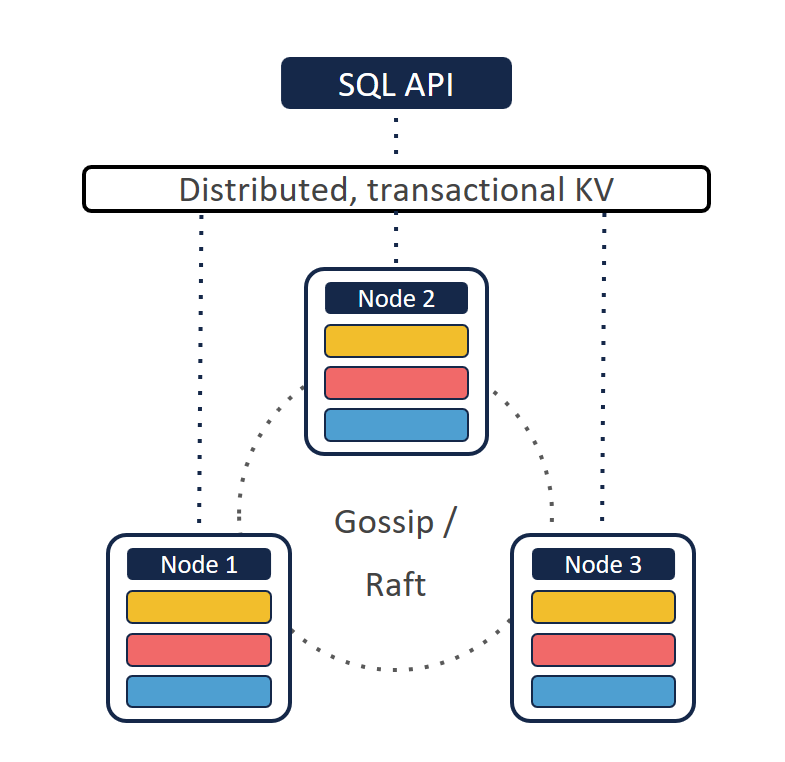
\includegraphics[width=0.5\textwidth]{resources/crdb-arhitecture-overview.png}
\end{center}
\caption{Arhitekturni pregled \cite{CRDB-2017}}
\label{img_crdb_arhitecture_overview}
\end{figure}

\subsubsection{Plasti}
Podatkovna baza CockroachDB je sestavljena iz petih plasti. Plasti med seboj delujejo kot črne škatle. Vsaka plast pa sodeluje le s plastjo neposredno nad in pod seboj.

\begin{enumerate}
    \item \textbf{SQL plast:} Prevede SQL poizvedbe v operacije tipa ključ-vrednost (KV).
    \item \textbf{Transakcijska plast:} Omogoča atomične spremembe nad večjim šte\-vi\-lom KV operacij.
    \item \textbf{Porazdelitvena plast:} Predstavi replicirana KV območja kot eno entiteto.
    \item \textbf{Replikacijska plast:} Konsistentno in sinhrono replicira KV obsege v gruči.
    \item \textbf{Shranjevalna plast:} Izvaja bralne in pisalne operacije na disku.
\end{enumerate}

\subsection{SQL plast}

SQL plast predstavlja vmesnik med podatkovno bazo ter ostalimi aplikacijami.  Podatkovna baza CockroachDB implementira velik del SQL standarda \cite{CRDB-sql-standard}. Zunanje aplikacije komunicirajo preko PostgreSQL žičnega protokola (angl. PostgreSQL wire protocol) \cite{psql-wire-protocol}. To omogoča enostavno povezavo med zunanjimi aplikacijami in kompatibilnost z obstoječimi gonilniki, orodji ter ORM-ji.

Poleg tega so vsa vozlišča v CockroachDB gruči simetrična, kar pomeni, da se lahko aplikacija poveže na katero koli vozlišče. To vozlišče obdela zahtevek oziroma ga preusmeri na vozlišče, katero ga zna obdelati. To omogoči enostavno porazdelitev bremena.

Ko vozlišče prejme SQL zahtevek, ga najprej razčleni v abstraktno sintaksno drevo. Potem CockroachDB začne s pripravo poizvedovalnega plana. V tem koraku CockroachDB preveri tudi semantično pravilnost poizvedb, nato vse operacije prevedene v KV operacije ter transformira podatke v binarno obliko. S pomočjo poizvedovalnega plana transakcijska plast nato izvede vse operacije. Kot primer poglejmo poenostavljeno stanje KV hrambe (tabela \ref{tbl_crdb_sql_kv_mapping}) po izvedbi naslednjih SQL stavkov:

\begin{listing}[H]
\begin{minted}{vim}
    CREATE TABLE customer (
        name STRING PRIMARY KEY,
        address STRING,
        url STRING
    );
    INSERT INTO customer VALUES (
        'Apple',
        '1 Infinite Loop, Cupertino, CA',
        'http://apple.com/'
    );
\end{minted}
\label{sql-example-sql-mapping}
\end{listing}

\begin{table}[H]
\begin{center}
\begin{tabular}{ l|l } 
\textbf{ključ} & \textbf{vrednost} \\
\hline
/system/databases/mydb/id & 51 \\
/system/tables/customer/id & 42 \\ 
/system/desc/51/42/address & 69 \\ 
/system/desc/51/42/url & 66 \\
/51/42/Apple/69 & 1 Infinite Loop, Cupertino, CA \\
/51/42/Apple/66 & http://apple.com/ \\
\end{tabular}
\end{center}
\caption{Poenostavljen primer preslikave SQL v KV model \cite{CRDB-design}. V podatkovni bazi \texttt{mydb} se nahaja tabela \texttt{customer}, katera ima poleg primarnega ključa še dva stolpca \texttt{address} in \texttt{url}. Zadnja dva zapisa v tabeli predstavljata eno vrstico v tabeli \texttt{customer} s primarnim ključem \texttt{Apple}.}
\label{tbl_crdb_sql_kv_mapping}
\end{table}

\subsection{Transakcijska plast}
Podatkovna baza CockroachDB je konsistentna. To dosega tako, da transakcijska plast implementira celotno semantiko ACID transakcij. Vsak stavek je obravnavan kot svoja transakcija, za katero stoji \texttt{COMMIT}. Temu pravimo način avtomatskega potrjevanja transakcij (angl. autocommit mode). Transakcije pa niso omejene samo na en stavek, določeno tabelo, obseg ali vozlišče in delujejo preko celotne gruče. To dosežejo z dvofaznim potrditvenim postopkom (angl. two-phase commit):

\begin{enumerate}
    \item \textbf{Faza 1:} Vsaka transakcija najprej kreira transakcijski zapis s statusom "v teku" (angl. pending). To je podatkovna struktura, katera nosi transakcijski ključ in status transakcije. Sočasno se za pisalne operacije kreira pisalni namen (angl. write intent). Pisalni namen je v osnovi MVCC vrednost, označena z zastavico \texttt{<intent>} in kazalcem na transakcijski zapis. Primer MVCC shrambe je prikazan v tabeli \ref{tbl_crdb_mvcc_store}.
    \item \textbf{Faza 2:} V kolikor je transakcijski zapis spremenjen v status prekinjeno (angl. aborted), se transakcija ponovno izvrši, če pa so izpolnjeni vsi pogoji, se transakcija potrdi. Status v transakcijskem zapisu se spremeni v potrjeno (angl. commited).
    \item \textbf{Faza 3 (asinhrono):} Ko se transakcija konča, se vsem potrjenim pisalnim namenom odstrani zastavico \texttt{<intent>} in kazalec na transakcijski zapis. Nepotrjeni pisalni nameni se samo izbrišejo. To se izvede asinhrono, zato vse operacije, preden kreirajo pisalni namen, preverijo obstoječi pisalni namen s transakcijskim zapisom in ga ustrezno upoštevajo.
\end{enumerate}

\begin{table}[H]
\begin{center}
\begin{tabular}{ l|l|l } 
\textbf{ključ} & \textbf{čas} & \textbf{vrednost} \\
\hline
A$<$intent$>$ & 500 & nepotrjena vrednost \\
A & 400 & trenutna vrednost \\ 
A & 322 & stara vrednost \\ 
A & 50 & prvotna vrednost \\
B & 100 & vrednost B \\
\end{tabular}
\end{center}
\caption{Primer MVCC shrambe s pisalnim namenom na ključu A \cite{CRDB-blog-transaction-isolation}.}
\label{tbl_crdb_mvcc_store}
\end{table}

Podatkovna baza CockroachDB privzeto podpira najvišji standardni SQL izolacijski nivo, to je \textit{serializable}. Ta nivo ne dopušča nikakršnih anomalij v podatkih. Če obstaja možnost anomalije, se transakcija ponovno izvede. Alternativno podpira tudi zastareli nestandardni izolacijski nivo \textit{snapshot}.

    
\subsection{Porazdelitvena plast}

Vsi podatki v gruči so na voljo preko katerega koli vozlišča. CockroachDB shranjuje podatke v urejeno vrsto tipa ključ-vrednost. Ta podatkovna stru\-ktu\-ra je namenjena shranjevanju tako sistemskih, kakor tudi uporabniških podatkov. Z nje CockroachDB razbere, kje se nahaja podatek in vrednost samega podatka. Podatki so razdeljeni na koščke, katere imenujemo obsegi (angl. ranges). Obsegi so urejeni koščki podatkov, preko katerih lahko CockroachDB hitro in učinkovito izvede \textit{lookup} in \textit{scan} operacije.

Lokacija vseh obsegov je shranjena v dvo-nivojskem indeksu. Ta indeks na prvem nivoju sestavlja meta obseg (angl. meta range) imenovan \texttt{meta1}, kateri kaže na meta obseg, na drugem nivoju pa obseg, imenovan \texttt{meta2}. Meta obseg \texttt{meta2} kaže na podatkovne obsege.

Ko vozlišče prejme zahtevek, v meta obsegih poišče vozlišče, katero hrani obseg v najemu (angl. range lease) ter preko tega vozlišča izvede zahtevek. Meta obsegi so predpomnjeni, zato se lahko zgodi, da kažejo na napačno vozlišče. V tem primeru se vrednosti meta obsegov posodobijo.

Privzeto je velikost podatkovnega obsega omejena na 64 MiB. To omogoča lažji prenos obsega med vozlišči, poleg tega pa je obseg dovolj velik, da lahko hrani nabor urejenih podatkov, kateri so bolj verjetno dostopani skupaj. Če obseg preseže velikost 64 MiB, se razdeli v dva 32 MiB podatkovna obsega. Ta dvo-nivojska indeksna struktura omogoča, da naslovimo do \(2^{(18 + 18)} = 2^{36}\) obsegov. Vsak obseg pa privzeto naslavlja \(2^{26}B = 64 MiB\) pomnilniške prostora. Teoretično lahko podatkovna baza CockroachDB s privzetimi nastavitvami naslovi do \(2^{(36+26)}B = 4 EiB\) podatkov. 

\subsection{Replikacijska plast}

Replikacijska plast skrbi za kopiranje podatkov med vozlišči in jih ohranja v konsistentnem stanju. To doseže preko soglasnega algoritma (angl. consensus algorithm) Raft \cite{raft-vs-paxos}. Ta algoritem zagotovi, da se večina vozlišč v gruči strinja z vsako spremembo v podatkovni bazi. S tem, kljub odpovedi posameznega vozlišča, ohrani podatke v konsistentnem stanju, poleg tega pa zagotovi nemoteno delovanje podatkovne baze (visoko razpoložljivost).

Število vozlišč, ki lahko odpove, ne da bi s tem vplivalo na delovanje podatkovne baze, je enako:
\[(r - 1)/2 = f \text{, če}\ r = 3, 5, 7, ...\ \text{in}\ r <= N\]
Kjer je \(N\) število vseh vozlišč v gruči; \(r\) faktor replikacije oz. liho število, večje ali enako tri in manjše ali enako številu vseh vozlišč v gruči; ter \(f\) maksimalno število vozlišč, ki še lahko odpove, brez da bi vplivalo na delovanje podatkovne baze. Na primer če je replikacijski faktor \(r = 3\), pomeni, da za vsak obseg obstajajo 3 replike, shranjene na treh različnih vozliščih. Gruča posledično lahko tolerira odpoved enega vozlišča \(f = 1\).

Za vsak obseg obstaja Raft skupina, kjer je eno vozlišče, ki vsebuje repliko, označeno kot "vodja". Vodja je izvoljen in koordinira vse pisalne zahtevke za določen obseg. V idealnih pogojih je vodja Raft skupine tudi najemnik obsega (angl. leaseholder).

\subsection{Shranjevalna plast}

CockroachDB za shranjevanje uporablja KV shrambo RocksDB \cite{rocksdb-home}. Ker KV shramba RocksDB omogoča transakcije, to bistveno olajša implementacijo ACID transakcij v podatkovni bazi CockroachDB.

CockroachDB uporablja MVCC pristop in hrani več verzij vsakega podatka. Podatkovna baza CockroachDB preko MVCC pristopa omogoča poizvedbe v zgodovino \texttt{SELECT...AS OF SYSTEM TIME}. Privzeto stare verzije podatkov pretečejo po 24 urah in so počiščene iz shrambe. Primer poizvedbe po zgodovinskih podatkih:

\begin{listing}[H]
\begin{minted}{vim}
    SELECT name, balance
    FROM accounts
        AS OF SYSTEM TIME '2016-10-03 12:45:00'
    WHERE name = 'Edna Barath';
\end{minted}
\label{sql-example-as-of-system-time}
\end{listing}

\section{Lastnosti}
Razvoj podatkovne baze CockroachDB je bil usmerjen prvotno v funkcionalnosti in šele kasneje v optimizacije. Tako je verzija 1.0.0 (maj 2017) omogočila razvijalcem večino potrebnih funkcionalnosti, kot so poizvedovalni jezik SQL porazdeljene poizvedbe, ACID transakcije, visoka razpoložljivost preko avtomatske replikacije in enostavno namestitev. Verzija 2.0.0 (april 2018) pa je prinesla zmogljivostne izboljšave ter boljšo kompatibilnost s podatkovno bazo PostgreSQL.

\subsection{Enostavnost}
Podatkovna baza CockroachDB stremi k enostavnosti upravljanja in vzdr\-že\-van\-ja. Večina kompleksnosti glede zagotavljanja visoke razpoložljivosti, avtomatske obnove vozlišč, usmerjanja porazdeljenih poizvedb in izenačevanja obremenitve je skoraj v celoti skrita končnemu uporabniku. Izogiba se zunanjim odvisnostim in je na voljo kot ena sama binarna datoteka. Minimalno je za zagon gruče potrebno na vsakem vozlišču zagotoviti sinhronizacijo ure, priporočena je uporaba zunanje Google NTP storitve, ter kopirati CockroachDB binarno datoteko na vsako vozlišče in jo zagnati.

\subsection{Uporabniški vmesnik in nadzorovanje}
Poleg podatkovne baze CockroachDB vsebuje tudi spletni administratorski vmesnik, ki je prikazan na sliki \ref{img_crdb_admin_ui}. Administratorski vmesnik nudi vizualizacije raznih časovnih metrik o delovanju posameznih vozlišč, kakor tudi celotne gruče. Omogoča pregled dnevnikov in pripomore k lažjemu odkrivanju težav v gruči. CockroachDB omogoča tudi izvoz metrik v odprtokodno rešitev Prometheus, katera nam omogoča shrambo, obdelavo, vizualizacije in obveščanje nad časovnimi vrstami.

\begin{figure}[H]
\begin{center}
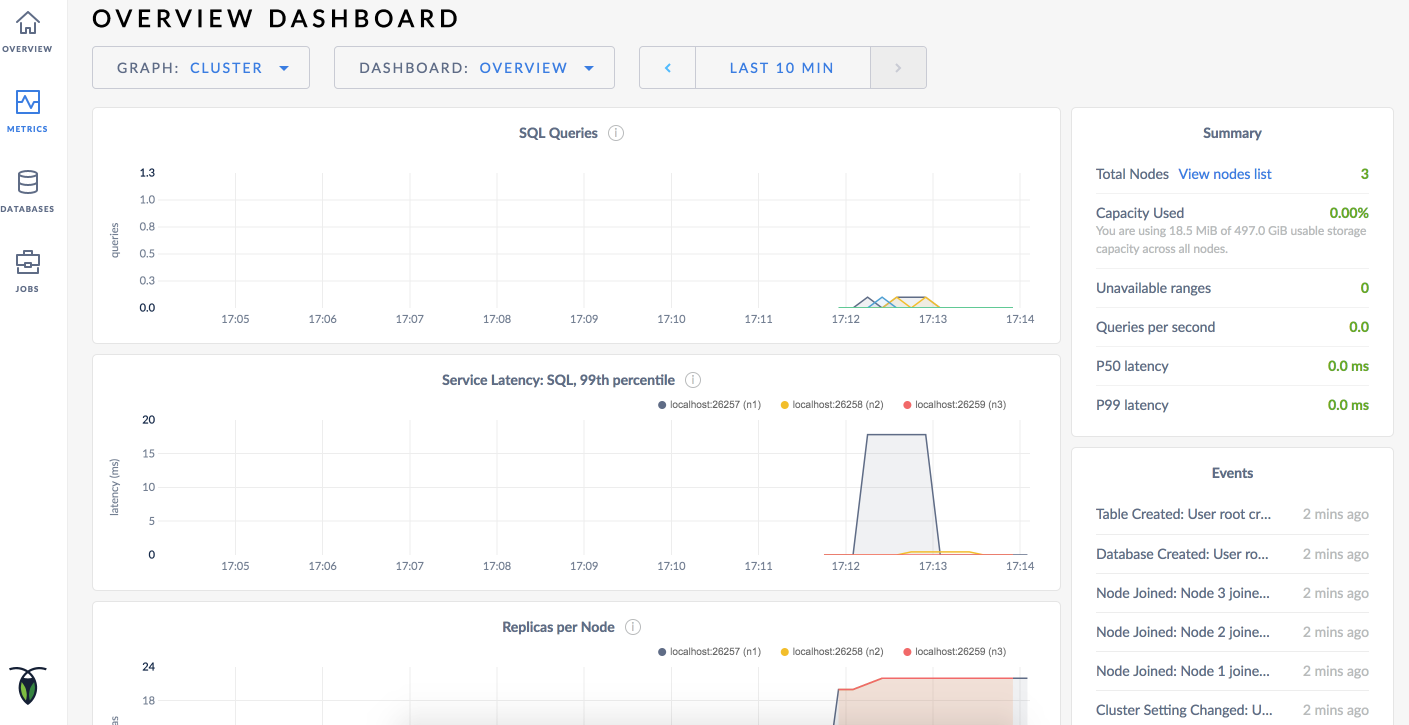
\includegraphics[width=1\textwidth]{resources/crdb_admin_ui.png}
\end{center}
\caption{Primer spletnega administratorskega vmesnika podatkovne baze CockroachDB.}
\label{img_crdb_admin_ui}
\end{figure}

\subsection{Podpora standardom SQL}
CockroachDB, kakor večina relacijskih podatkovnih baz, podpira podmnožico SQL standarda \cite{CRDB-sql-standard}. Poleg tega implementira nekatere najpogostejše raz\-ši\-rit\-ve, razširitve, specifične za PostgreSQL, ter svoje razširitve. V spodnjih podpoglavjih bomo v grobem opisali, kaj od jezika SQL ponuja CockroachDB, bolj podroben opis pa se nahaja v uradni dokumentaciji \cite{CRDB-sql-features}.

\subsubsection{Podatkovni tipi}
CockroachDB podpira naslednje podatkovne tipe:

\begin{itemize}
    \item \textbf{Celoštevilčni}: \texttt{INT} in \texttt{SERIAL} (avtomatsko kreirana unikatna številka)
    \item \textbf{Decimalni}: \texttt{DECIMAL} in \texttt{FLOAT}
    \item \textbf{Textovni}: \texttt{STRING} in \texttt{COLLATE} (podobno kot \texttt{STRING}, vendar upošteva specifike jezika)
    \item \textbf{Datumski in časovni}: \texttt{DATE}, \texttt{TIME}, \texttt{INTERVAL} (časovni interval) in\\\texttt{TIMESTAMP} (datum in čas)
    \item \textbf{Ostali}: \texttt{ARRAY}, \texttt{BOOL}, \texttt{BYTES}, \texttt{INET} (IPv4 in IPv6 naslovi), \texttt{JSONB} in\\\texttt{UUID} (128-bitna heksadecimalna vrednost)
\end{itemize}

\noindent Poleg zgoraj naštetih podatkovnih tipov ima vsak podatkovni tip zaradi kompatibilnosti s standardnim SQL jezikom še nekaj psevdonimov. CockroachDB ne podpira podatkovnih tipov, kot so \texttt{XML}, \texttt{UNSIGNED INT} ter \texttt{SET} in \texttt{ENUM}.

\newpage
\subsubsection{Shema}
CockroachDB podpira vse standardne ukaze za kreiranje, spreminjanje in odstranjevanje baz, tabel, stolpcev, omejitev, indeksov in pogledov. Od podatkovnih omejitev podpira vse standardne, to so: \texttt{PRIMARY KEY}, \texttt{NOT NULL}, \texttt{UNIQUE}, \texttt{CHECK}, \texttt{FOREIGN KEY} in \texttt{DEFAULT}. Omejitev \texttt{PRIMARY KEY} lahko nastavimo samo ob kreiranju tabele in je kasneje ne moremo spreminjati. Če omejitve \texttt{PRIMARY KEY} ne nastavimo v času kreiranja tabele, CockroachDB v ozadju sam kreira skriti stolpec s tipom \texttt{UUID}, saj je ta pomemben za samo delovanje podatkovne baze.

Poizvedovanje sheme je na voljo na standardni način, preko virtualne sheme \texttt{information\_schema}.

Prožilci (angl. triggers) še niso podprti in tudi ne načrtovani za naslednje verzije.

\subsubsection{Transakcije}
CockroachDB podpira ACID transakcije, katere so lahko porazdeljene preko celotne gruče. Privzeto transakcije uporabljajo najvišji izolacijski nivo \texttt{SERI\-ALIZABLE}, omogočajo pa še zastareli izolacijski nivo \texttt{SNAPSHOT}. Ostali standardni izolacijski nivoji niso podprti.

\subsubsection{Tabelarični izrazi}
CockroachDB podpira referenciranje tabel, pogledov, poizvedb, tabelaričnih funkcij in CTE-jev (angl. common table expressions). Podpora za CTE-je je le osnovna, referenciramo jih lahko samo enkrat, poleg tega pa jih ni mogoče uporabiti v pogledih.

Od pod-poizvedb (angl. sub-queries) omogoča le nekorelirane pod-poiz\-vedbe. Nekorelirane pod-poizvedbe so poizvedbe, katere ne referencirajo nadrejenih poizvedb. Običajno je možno korelirano pod-poizvedbo spremeniti v nekorelirano z uporabo stične operacije:

\begin{listing}[H]
\begin{minted}{vim}
    # Z uporabo korelirane pod-poizvedbe (nepodprto)
    SELECT c.name
    FROM customers c
    WHERE EXISTS(
        SELECT *
        FROM orders o
        WHERE o.customer_id = c.id
    );

    # Z uporabo stične operacije (podprto)
    SELECT DISTINCT ON(c.id) c.name
    FROM customers c CROSS JOIN orders o
    WHERE c.id = o.customer_id;
\end{minted}
\label{code-correlated-sub-queries}
\end{listing}

Od stičnih operacij CockroachDB omogoča \texttt{INNER JOIN}, \texttt{LEFT JOIN},\\\texttt{RIGHT JOIN}, \texttt{FULL JOIN} in \texttt{CROSS JOIN}. Stične operacije še niso optimizirane. Da bi te dosegle optimalno delovanje, je zelo pomemben optimalni zapis poizvedbe, ustrezni filtri in morebitna uporaba eksperimentalne zastavice \texttt{SET experimental\_force\_lookup\_join = true}.

\subsubsection{Operatorji, skalarni izrazi, logični izrazi in funkcije}
CockroachDB implementira večji del standardnih operatorjev, skalarnih izrazov, logičnih izrazov ter funkcij. Podpira poizvedovanje po tipu JSON, omogoča iskanje s POSIX regularnimi izrazi ter implementira agregacijske funkcije (funkcije, katere se izvedejo nad posamezno skupino ob uporabi \texttt{GROUP BY}) in okenske funkcije (\texttt{OVER()}).

Uporabniške funkcije niso podprte in tudi ne načrtovane za naslednje verzije. Shranjene procedure so načrtovane za eno od naslednjih verzij.

\subsection{Licenca}

CockroachDB je odprtokodna in zastonjska podatkovna baza. Večino potrebnih funkcionalnosti omogoča zastonjska različica, poleg tega pa ponuja tudi poslovno licenco. Poslovna licenca strankam omogoča:

\begin{itemize}
    \item svetovanje;
    \item tehnično pomoč;
    \item geografsko porazdelitev podatkov na nivoju ene vrstice (podatki so blizu uporabnika);
    \item vizualizacijo geografsko porazdelitve gruče na zemljevidu;
    \item nadzor dostopa na nivoju skupin in
    \item porazdeljeno kreiranje in obnovo varnostnih kopij.
\end{itemize}

\subsection{Podprta orodja, gonilniki, ORM-ji in skupnost}

Podatkovna baza CockroachDB implementira standardni SQL \cite{CRDB-sql-standard}, za komunikacijo med odjemalcem in strežnikom pa uporablja PostgreSQL žični protokol, kar omogoča dobro kompatibilnost z obstoječimi PostgreSQL komponentami.

Na uradni spletni dokumentaciji je za jezike Go, Java, .NET, C++, NodeJS, PHP, Python, Ruby, Rust, Clojure ter Elixir objavljen seznam podprtih gonilnikov in ORM-jev. Za vse gonilnike CockroachLabs v času pisanja zagotavlja le beta podporo \cite{CRDB-meta-drivers-orms}.

Od orodij za upravljanje s podatkovno bazo nam CockroachLabs ponuja konzolno aplikacijo \texttt{cockroach sql}. Od grafičnih orodij nudijo beta podporo \cite{CRDB-meta-vizualizers} za pgweb \cite{pgweb-home}, dbglass \cite{dbglass-home}, Postico \cite{postico-home}, PSequel \cite{psequel-home}, TablePlus \cite{tableplus-home} in Valentina studio \cite{valentinastudio-home}.

Orodje pgweb, ki je bilo primarno razvito za podatkovno bazo PostgreSQL, ima trenutno najbolj aktivno skupnost, je odprtokodno in podpira vse glavne operacijske sisteme (Windows, OSX in Linux). Do aplikacije dostopamo preko spletnega brskalnika. Orodje pgweb podpira funkcionalnosti, kot so:

\begin{itemize}
    \item pregled podatkovne baze in sheme;
    \item izvedba in analiza SQL poizvedb;
    \item zgodovina poizvedb;
    \item izvoz podatkov v formatu CSV, JSON in XML.
\end{itemize}

Izvirna koda podatkovne baze CockroachDB je javno dostopna preko GitHub repozitorija \texttt{cockroachdb/cockraoch} \cite{cockroachdb/cockroach}. Projekt ima aktivno skupnost in mu trenutno sledi približno 14 tisoč navdušencev. Poleg GitHub repozitorija, kjer se odvija ves razvoj, vodenje nalog in pomoč, CockroachLabs vodi še spletno stran \cite{CRDB-home} (dokumentacija, form, blog, mediji), Gitter kanal \cite{CRDB-gitter} in Docker repozitorij \cite{CRDB-docker}.

\chapter{Primerjalna analiza zmogljivosti CockroachDB}

Primerjalna analiza zmogljivosti (angl. performance benchmarking) je postopek za primerjavo enega sistema z ostalimi podobnimi sistemi. V našem primeru smo z orodjem YCSB primerjali podatkovni bazi CockroachDB ter PostgreSQL z nameščeno razširitvijo Citus (v nadaljevanju samo Citus). 

Za primerjavo s Citus smo se odločil zaradi lažje izvedbe ter bolj primerljivih rezultatov. Obe podatkovni bazi CockroachDB in Citus sta po nekaterih lastnostih zelo podobni. Obe podatkovni bazi implementirata standardni SQL ter komunicirata preko PostgreSQL žičnega protokola. Podatkovno bazo smo nekoliko bolj podrobno opisali v poglavju \ref{benchmarking/citus}.

Za orodje YCSB smo se odločili, saj podpira vmesnik JDBC, katerega podpirata tudi obe podatkovni bazi, poleg tega pa je enostavno za uporabo. Orodje YCSB smo bolj podrobno opisal v poglavju \ref{YCSB_about}. Ob iskanju najprimernejšega orodja smo pregledali še naslednja orodja:

\begin{itemize}
    \item \textbf{TPC:}\\ TPC (angl. transaction processing performance council) \cite{TPC-home} je neprofitna organizacija, ki nudi preverljive podatke TPC zmogljivostnih analiz podatkovnih baz. TPC definira več različnih standardnih testov, ki simulirajo različne realne obremenitve. Ti testi so natančno opisani, strogo omejeni in kompleksni. Primer testa za transakcijske obremenitve je test TPC-C, ki simulira obremenitve v dobavnem skladišču. Primer za testiranje analitičnih obremenitev je test TPC-H, ki izvaja kompleksne poizvedbe za podporo pri odločanju.
    
    TPC testi so standardizirani in simulirajo realne obremenitve za dolo\-čene problemske domene. Ti testi bi bili najbolj primerni, vendar pa so zelo točno definirani, kompleksni in težki za izvedbo, zato jih v diplomskem delu nismo izvedli. Uradnih TPC testov za podatkovno bazo CockroachDB še ni.
    \item \textbf{pgbench:}\\ Je enostavno orodje, namenjeno zmogljivostni analizi PostgreSQL podatkovnih baz \cite{pgbench}. Simulira transakcijsko obremenitev, podobno zastarelemu testu TPC-B. Test TPC-B simulira obremenitve v bančni\-štvu. 
    
    Orodje pgbench v času testiranja še ni bilo kompatibilno s podatkovno bazo CockroachDB.
    \item \textbf{cockroachdb/loadgen:}\\ Je skupek orodij, namenjenih zmogljivostni analizi CockroachDB podatkovne baze \cite{cockroachdb/loadgen}. Orodje vsebuje nabor testov, ki generirajo TPC-C, TPC-H, YCSB in KV obremenitve. Te orodja CockroachLabs interno uporablja za zmogljivostno primerjavo med posameznimi verzijami podatkovne baze CockroachDB. Kasneje je bil objavljen članek, kjer so primerjali rezultate TPC-C obremenitve med podatkovnima bazama CockroachDB in Amazon Aurora \cite{CRDB-tpcc-vs-aurora}.

    Orodje je enostavno, vendar pa je slabo dokumentirano in ne omogoča zmogljivostne analize podatkovne baze PostgreSQL.
    \item \textbf{Apache JMeter:}\\ Je orodje, namenjeno izvajanju raznih obremenitvenih testov \cite{jmeter}. Orod\-je omogoča izvajanje poljubnih obremenitev podatkovnih baz preko JDBC vmesnika.
    
    Orodje je zelo konfigurabilno, vendar pa ne omogoča v naprej definiranih obremenitvenih testov. Zaradi kompleksnosti je težko za uporabo.
    \item \textbf{YCSB:}\\ YCSB (angl. Yahoo! Cloud Serving Benchmark) je orodje, namenjeno za primerjavo zmogljivostnih metrik med raznimi podatkovnimi bazami \cite{brianfrankcooper/YCSB}. Orodje smo podrobneje opisali v poglavju \ref{YCSB_about}.
\end{itemize}

V naslednjih podpoglavjih bomo opisali točen postopek, s katerim smo izvedli primerjalno analizo. Opisali bomo strojno arhitekturo, pripravo posameznih konfiguracij, pripravo podatkov in samo testiranje. Na koncu bomo predstavili rezultate zmogljivostne analize ter naše ugotovitve.

\section{Hipoteze}
Pred začetkom izvajanja primerjalne analize smo postavili naslednje hipoteze:
\begin{enumerate}
    \item CockroachDB bo na enem vozlišču nekoliko počasnejši od PostgreSQL podatkovne baze.
    \iffalse
    Razlog za to hipotezo je, da je CockroachDB na trgu dobro leto in še ni dokončno optimiziran, medtem ko je PostgreSQL na trgu dobrih 20 let.
    \fi
    \item CockroachDB bo zaradi linearne skalabilnosti na treh vozliščih skoraj trikrat bolj zmogljiv.
\end{enumerate}

\section{Testno okolje}
Testno okolje sestavljajo štiri vozlišča, označena z \texttt{n0}, \texttt{n1}, \texttt{n2} in \texttt{n3}. Specifikacije strojne opreme so opisane v tabeli \ref{tbl_benchmarking_nodes_hw}. Vsa vozlišča imajo nameščen Ubuntu 16.04 LTS, Docker 18.03.0-ce ter ntpd, ki je konfiguriran glede na produkcijska priporočila  CockroachDB podatkovne baze \cite{CRDB-ntpd-configuration}.

Veliko časa smo vložili v samo postavitev testnega okolja. Zaradi natančnosti testov smo bili pozorni, da smo odpravili čim več spremenljivk, ki bi lahko vplivale na končne rezultate.
Vsa štiri vozlišča so med seboj povezana preko gigabitnega Ethernet omrežja v Docker Swarm \cite{Docker-Swarm-Mode} gručo. Vozlišče \texttt{n0} je v vlogi vodje, vozlišča \texttt{n1}, \texttt{n2} in \texttt{n3} pa so v vlogi delavcev. Za uporabo Docker Swarm tehnologije smo se odločili zaradi enostavnosti postavitve testnega okolja, avtomatizacije in izvedbe samih testov ter lažje ponovljivosti testov.

Ker tehnologije Docker še nismo dobro poznali, smo imeli v fazi prototipiranja težave pri zmogljivosti. Izkazalo se je, da je bil ključen problem v tem, da nismo uporabili podatkovnih nosilcev (angl. data volumes) \cite{docker-storage-layers}.

\begin{table}[H]
\begin{center}
\begin{tabular}{ l|l|l|l } 
    & \textbf{procesor} & \textbf{pomnilnik} & \textbf{trdi disk} \\
\hline
n0 & \makecell[l]{Intel Core2 Quad CPU Q9400\\št. jeder: 4\\frekvenca: 2,66 GHz\\predpomnilnik: 6 MB} & 4 GB & \makecell[l]{SAMSUNG HD753LJ\\velikost: 750 GB\\frekvenca: 7200 RPM\\predpomnilnik: 32 MB} \\
\hline
n1 & \makecell[l]{Intel Core i5 CPU 650\\št. jeder: 4\\frekvenca: 3,20 GHz\\predpomnilnik: 4 MB} & 4 GB & \makecell[l]{WDC WD10EARS-22Y5B1\\velikost: 1 TB\\frekvenca: 5400 RPM\\predpomnilnik: 64 MB} \\
\hline
n2 & \makecell[l]{Intel Core i7-3770\\št. jeder: 8\\frekvenca: 3,40 GHz\\predpomnilnik: 8 MB} & 8 GB & \makecell[l]{ST500DM002-1BD142\\velikost: 500 GB\\frekvenca: 7200 RPM\\predpomnilnik: 16 MB} \\
\hline
n3 & \makecell[l]{Intel Core i5-2400\\št. jeder: 4\\frekvenca:  3,10 GHz \\predpomnilnik: 6 MB} & 4 GB & \makecell[l]{Hitachi HDS721050CLA662\\velikost: 500 GB\\frekvenca: 7200 RPM\\predpomnilnik: 16 MB} \\
\end{tabular}
\end{center}
\caption{Specifikacije strojne opreme, ki se razlikujejo med posameznimi vozlišči.}
\label{tbl_benchmarking_nodes_hw}
\end{table}

\subsection{Odjemalec}
Vozlišče n0 je v vlogi odjemalca. Na njem teče program, ki zažene podatkovno bazo, obnovi podatke, izvaja teste in beleži rezultate. Podroben opis delovanja odjemalca se nahaja v poglavju \ref{YCSB_benchmarking_steps}.

\subsection{Strežnik}
V vlogi strežnika so vozlišča \texttt{n1}, \texttt{n2} in \texttt{n3}. Na njih teče ali CockroachDB ali PostgreSQL z nameščeno razširitvijo Citus. V primeru, da gre za konfiguracijo z enim vozliščem, podatkovna baza teče na vozlišču \texttt{n2}.

\section{Razširitev Citus}
\label{benchmarking/citus}
Citus je razširitev za podatkovno bazo PostgreSQL \cite{citus}. Omogoča enostavno horizontalno skaliranje podatkov za več najemniške (angl. multi tenant) aplikacije in obdelavo analitičnih podatkov v realnem času (angl. real time analytics). Uporaba razširitve Citus ni primerna, če:
\begin{itemize}
    \item nam zadošča le eno vozlišče;
    \item poizvedbe vračajo ogromno podatkov in
    \item ne potrebujemo analitike v realnem času.
\end{itemize}

Razširitev Citus nam je voljo kot odprtokodna razširitev, plačljiva različi\-ca in storitev (DBaaS). Plačljiva različica poleg fukcionalnosti odprtokodne raz\-širitve ponuja še nekaj dodatne funkcionalnosti in 24-urno podporo strankam.

Za primerjavo s Citus smo se odločili predvsem zaradi enostavnosti izvedbe primerjalne zmogljivostne analize. Obe podatkovni bazi, CockroachDB in Citus, temeljita na podatkovni bazi PostgreSQL. Obe komunicirata preko PostgreSQL žičnega protokola. Prav tako pa enostavna YCSB shema, katero smo opisali v naslednjem poglavju \ref{YCSB_about}, dobro spada v kontekst več najemniških aplikacij.


\section{Orodje YCSB}
\label{YCSB_about}
YCSB \cite{brianfrankcooper/YCSB} je razširljiva in odprtokodna rešitev za primerjalno analizo zmogljivosti. Največkrat se uporablja za zmogljivostno analizo različnih NoSQL podatkovnih baz. Podpira veliko število različnih podatkovnih baz, kot so  Mongo, Couchbase, S3, Redis itd. Poleg tega pa podpira tudi vmesnik JDBC, preko katerega smo primerjali podatkovno bazo CockroachDB ter Citus. YCSB nudi nekaj vnaprej definiranih obremenitev, katere smo tudi uporabili v naši primerjalni analizi zmogljivosti \cite{YCSB-core-workloads}:
\begin{itemize}
    \item \textbf{A} - Obremenitev je sestavljena iz 50 \% \texttt{SELECT} in 50 \% \texttt{UPDATE} operacij.
    \item \textbf{B} - Obremenitev je sestavljena iz 95 \% \texttt{SELECT} in 5 \% \texttt{UPDATE} operacij.
    \item \textbf{C} - Obremenitev je sestavljena iz 100 \% \texttt{SELECT} operacij.
    \item \textbf{D} - Obremenitev je sestavljena iz 95 \% \texttt{SELECT} in 5 \% \texttt{INSERT} operacij, pri čemer bere vedno zadnje vstavljene vrstice.
    \item \textbf{F} - Obremenitev je sestavljena iz 50 \% \texttt{SELECT} in 50 \% \texttt{SELECT} - \texttt{UPDATE} operacij.
\end{itemize}

Izbira vrstice je pri A, B, C in F obremenitvah porazdeljena preko Zipf porazdelitvene funkcije. Zipfov zakon pravi, da je najbolj verjetna vrednost približno dvakrat bolj verjetna od druge najbolj verjetne vrednosti in trikrat bolj verjetna od tretje najbolj verjetne vrednosti \cite{zipfs-law}.

Orodje YCSB vrača rezultate v enostavni tekstovni obliki. Od rezultatov vrne skupni čas trajanja, prepustnosti (enačba \ref{eq:throughput}) ter agregirano število vseh operacij in različne podatke o latencah (enačba \ref{eq:latency}). Od latence vrača povprečno vrednost, minimalno in maksimalno vrednost ter 95 in 99 percentil.

\begin{equation} \label{eq:throughput}
throughput = 1000 * total\_operations / total\_duration\_ms
\end{equation}

\begin{equation} \label{eq:latency}
latency = operation\_end\_ms - operation\_start\_ms
\end{equation}

\section{Izvedba testiranja YCSB obremenitev}
\label{YCSB_benchmarking_steps}
Testiranje je potekalo iz odjemalca, torej vozlišča \texttt{n0}. Meritev je bilo veliko, zato smo pripravil program, s katerim smo izvedbo testiranja avtomatizirali. Program, s katerim smo testirali, je enostaven in ni prenosljiv. Izvorna koda in rezultati meritev so na voljo na GitHub repozitoriju \cite{matjazmav/diploma-ycsb}. V tem poglavju bomo opisal vse korake, ki so bili potrebni za izvedbo meritev.

\subsection{Namestitev programske opreme}
Na vozlišču \texttt{n0} smo namestili naslednjo programsko opremo:
\begin{itemize}
    \item YCSB (verzija 0.12.0) \cite{brianfrankcooper/YCSB} je orodje, namenjeno izvedbi zmogljivostne analize ter primerjavi med različnimi podatkovnimi bazami. Samo orodje smo bolj natančno opisali v poglavju \ref{YCSB_about}.
    \item Ansible (verzija 2.5.0) \cite{Ansible} je orodje za avtomatizacijo, uporabili smo ga zaradi lažjega konfiguriranja gruče preko SSH povezave.
    \item Go (verzija 1.10.1) \cite{Golang} je programski jezik, v katerem je napisan program za avtomatizacijo testiranja. Za programski jezik Go smo se odločili zaradi njegove enostavnosti.
\end{itemize} 

\subsection{Priprava podatkov}
\label{benchmarking-prepare-data}
Program za avtomatizacijo testiranja predpostavlja, da imajo vsa vozlišča na točno določeni lokaciji pripravljene podatke za obnovo fizične podatkovne baze. Pred vsakim testom se podatki kopirajo v začasno mapo, nad katero kasneje baza izvaja operacije. Po končanem testu se začasna mapa izbriše.

V spodnjih korakih je opisan postopek, po katerem smo pripravili podatke za vsako bazo ter za vsako konfiguracijo (eno vozlišče in tri vozlišča). Vse konfiguracijske datoteke, ki so uporabljene v spodnjih primerih, so na voljo na GitHub repozitoriju \texttt{matjazmav/diploma-ycsb} \cite{matjazmav/diploma-ycsb}.

\subsubsection{Citus}
\begin{enumerate}
    \item Z Docker Swarm konfiguracijsko skripto (\texttt{stacks/postgres-n1.yml}) smo pognal Citus podatkovno bazo na vozlišču \texttt{n2}.
    \item Na vozlišču \texttt{n2} smo ročno kreirali shemo, katero za svoje delovanje potrebuje orodje YCSB.
    \begin{listing}[H]
    \begin{minted}{vim}
        CREATE DATABASE ycsb;
        \c ycsb;
        CREATE TABLE usertable (
            YCSB_KEY VARCHAR(255) PRIMARY KEY,
            FIELD0 TEXT, FIELD1 TEXT,
            FIELD2 TEXT, FIELD3 TEXT,
            FIELD4 TEXT, FIELD5 TEXT,
            FIELD6 TEXT, FIELD7 TEXT,
            FIELD8 TEXT, FIELD9 TEXT
        );
    \end{minted}
    \label{code-ycsb-schema-postgres}
    \end{listing}
    \item Nato smo generirali podatke. V bazo na vozlišču \texttt{n2} smo z YCSB orodjem naložili 5 milijonov zapisov, kar na disku zasede približno 6 GB prostora.
    \begin{listing}[H]
    \begin{minted}{vim}
        ycsb load jdbc \
            -P workloads/workloada \
            -P configs/postgres-n1.properties \
            -p threadcount=16 \
            -p recordcount=5000000
    \end{minted}
    \label{code-ycsb-load-postgres}
    \end{listing}
    \item Podatkovno bazo smo varno ustavili ter naredili varnostno kopijo fizične podatkovne baze na disku.
    \item Nato smo z Docker Swarm konfiguracijsko skripto (\texttt{stacks/\\postgres-n3.yml}) pognali Citus podatkovno bazo na treh vozliščih.
    \item Na vozliščih \texttt{n1} in \texttt{n3} smo kreirali shemo, definirano v točki 2.
    \item Nato smo na vozlišču \texttt{n2} povezali še vozlišči \texttt{n1} ter \texttt{n3} in kreirali porazdeljeno tabelo. Podatki v tabeli \texttt{usertable} so se enakomerno porazdelili med vsa tri vozlišča.
    \begin{listing}[H]
    \begin{minted}{vim}
        \c ycsb;
        SELECT * FROM master_add_node('<n1 ip addr>', 5432);
        SELECT * FROM master_add_node('<n2 ip addr>', 5432);
        SELECT create_distributed_table('usertable', 'ycsb_key');
    \end{minted}
    \label{code-ycsb-add-node-citus}
    \end{listing}
    \item Po končani konfiguraciji smo bazo varno ustavili ter naredili varnostno kopijo podatkov na disku.
\end{enumerate}

\subsubsection{CockroachDB}
\begin{enumerate}
    \item Z Docker Swarm konfiguracijsko skripto (\texttt{stacks/\\cockroachdb-n1.yml}) smo pognali CockroachDB bazo na vozlišču \texttt{n2}.
    \item Na vozlišču \texttt{n2} smo ročno kreirali shemo, katero za svoje delovanje potrebuje orodje YCSB.
    \begin{listing}[H]
    \begin{minted}{vim}
        CREATE DATABASE ycsb;
        USE ycsb;
        CREATE TABLE usertable (
            YCSB_KEY VARCHAR(255) PRIMARY KEY,
            FIELD0 TEXT, FIELD1 TEXT,
            FIELD2 TEXT, FIELD3 TEXT,
            FIELD4 TEXT, FIELD5 TEXT,
            FIELD6 TEXT, FIELD7 TEXT,
            FIELD8 TEXT, FIELD9 TEXT
        );
    \end{minted}
    \label{code-ycsb-schema-cockroach}
    \end{listing}
    \item Nato smo generirali podatke. V bazo na vozlišču \texttt{n2} smo z YCSB orodjem naložili 5 milijonov zapisov, kar na disku zasede približno 6 GB prostora.
    \begin{listing}[H]
    \begin{minted}{vim}
        ycsb load jdbc \
            -P workloads/workloada \
            -P configs/cockroachdb-n1.properties \
            -p threadcount=16 \
            -p recordcount=5000000
    \end{minted}
    \label{code-ycsb-load-cockroach}
    \end{listing}
    \item Podatkovno bazo smo varno ustavili ter naredili varnostno kopijo fizične podatkovne baze na disku.
    \item Nato smo z Docker Swarm konfiguracijsko skripto (\texttt{stacks/\\cockroachdb-n3.yml}) pognali CockroachDB bazo na treh vozliščih.
    \item Baza je samodejno zaznala dve novi vozlišči in pričela avtomatsko z replikacijo podatkov na ostali dva vozlišči. Ko se je replikacija končala, smo bazo varno ustavili ter naredili varnostno kopijo fizične podatkovne baze na disku.
\end{enumerate}


\subsection{Program za avtomatizacijo}
Vozlišče \texttt{n0} je v vlogi odjemalca. Na njem teče program, ki za vse kombinacije parametrov (baza, število vozlišč, število sočasnih povezav) izvaja teste in beleži rezultate. Program predpostavlja, da obstajajo za vsako konfiguracijo vnaprej pripravljeni podatki na točno določenem mestu. Postopek za pripravo podatkov smo opisali v poglavju \ref{benchmarking-prepare-data}. Program v grobem za vsako kombinacijo parametrov izvede naslednje korake:
\begin{enumerate}
    \item obnovi vnaprej definirane podatke (\texttt{cp -a});
    \item zažene podatkovno bazo (\texttt{docker stack up});
    \item izvede YCSB test (\texttt{ycsb run jdbc ...});
    \item zabeleži rezultat v datoteko CSV;
    \item ustavi podatkovno bazo (\texttt{docker stack rm});
    \item počisti podatke (\texttt{rm -rf}).
\end{enumerate}

\noindent Koraki 2, 3, 4 in 5 se ponovijo za vsak tip obremenitve v natančno določenem vrstnem redu (A, B, C, F, D). Vrstni red obremenitev je pomemben \cite{YCSB-core-workloads}, ker obremenitve tipa A, B, C in F ne vstavljajo novih zapisov. Obremenitev tipa D pa vstavlja nove zapise, zato je po vsaki izvedbi potrebno obnoviti bazo na prvotno stanje. Zaradi morebitnih odstopanj smo vse teste ponovili trikrat.

\newpage
\section{Izvedba testiranja stičnih operacij}
Ker orodje YCSB izvaja le enostavne operacije nad eno tabelo, smo kasneje sami ročno preverili podporo za stične operacije.

\subsection{Priprava podatkov}
Osnova za te teste so nam bili podatki, katere smo predhodno pripravili. Priprava je opisana v poglavju \ref{benchmarking-prepare-data}. Poleg teh podatkov, ki vsebujejo le tabelo \texttt{usertable} (5 milijonov vrstic), smo kreirali še tabelo \texttt{ext} in vanjo zapisali 100 vrstic. Sam postopek kreiranja tabele \texttt{ext} je bil za Citus na treh vozliščih nekoliko drugačen, za ostale tri konfiguracije pa je bila uporabljena naslednja skripta:

\begin{listing}[H]
\begin{minted}{vim}
    CREATE TABLE ext (
        ycsb_key VARCHAR(255) PRIMARY KEY,
        value int not null );

    INSERT INTO ext
    SELECT
        ycsb_key,
        LTRIM(RIGHT(ycsb_key, 5), '0')::int % 10 AS value
    FROM usertable ORDER BY ycsb_key LIMIT 100;
\end{minted}
\label{benchmarking_joins_data}
\end{listing}

Za Citus podatkovno bazo je postopek nekoliko daljši. Ker ne moremo neposredno s porazdeljene tabele \texttt{usertable} kopirati v lokalno tabelo \texttt{ext}, moramo najprej kreirati začasno tabelo, podatke napolniti in potem iz začasne tabele podatke prestaviti v novo tabelo \texttt{ext}. To smo storili z naslednjo skripto:

\begin{listing}[H]
\begin{minted}{vim}
    CREATE TABLE ext (
        ycsb_key VARCHAR(255) PRIMARY KEY,
        value int not null );

    CREATE TEMPORARY TABLE tmp AS
    SELECT
        ycsb_key,
        LTRIM(RIGHT(ycsb_key, 5), '0')::int % 10 AS value
    FROM usertable ORDER BY ycsb_key LIMIT 100;

    INSERT INTO ext SELECT * FROM tmp;

    SELECT create_distributed_table('ext', 'ycsb_key');
\end{minted}
\label{benchmarking_joins_citus_data}
\end{listing}

\subsection{Izvedba testiranja in rezultati}
Testna poizvedba, ki smo jo uporabili na vseh štirih konfiguracijah, vrača 11 vrstic in 2 stolpca (\texttt{ycsb\_key} ter \texttt{field4}). Testna poizvedba je sledeča:

\begin{listing}[H]
\begin{minted}{vim}
    SELECT u.ycsb_key, u.field4
    FROM usertable u
    INNER JOIN ext e ON e.ycsb_key = u.ycsb_key
    WHERE e.value = 4; 
\end{minted}
\label{benchmarking_joins_query}
\end{listing}

Rezultati za podatkovno bazo CockroachDB so zelo slabi. Rezultati so predstavljeni v tabeli \ref{tbl_benchmarking_joins}. Podatkovna baza ne ugotovi, da tabela \texttt{ext} s filtrirnim pogojem omeji rezultat na 11 vrstic, zato začne združevati obe tabeli na 5 milijonih vrsticah. Obe poizvedbi smo po 1 minuti prekinili, po nekaj deset minutah pa je ukazna vrstica spet postala odzivna.

\begin{table}[H]
\begin{center}
\begin{tabular}{ l|l } 
\textbf{konfiguracija} & \textbf{čas [ms]} \\
\hline
Citus 1 vozlišče        & 66,336 \\
Citus 3 vozlišče        & 163,049 \\
CockroachDB 1 vozlišče  & (prekinjeno po 1 minuti)\\
CockroachDB 3 vozlišče  & (prekinjeno po 1 minuti)\\
\end{tabular}
\end{center}
\caption{Čas trajanja testne poizvedbe s stično operacijo glede na konfiguracijo.}
\label{tbl_benchmarking_joins}
\end{table}

\newpage

\section{Rezultati}
Vsi rezultati so na voljo na GitHub repozitoriju \texttt{matjazmav/diploma-ycsb} \cite{matjazmav/diploma-ycsb}. V mapi \texttt{results} se nahajajo datoteke z neobdelani podatki. Analizo rezultatov smo izvedli v Excel datoteki \texttt{results.xlsx}. Po analizi pa smo prišli do spodnjih rezultatov.

\begin{figure}[H]
\begin{center}
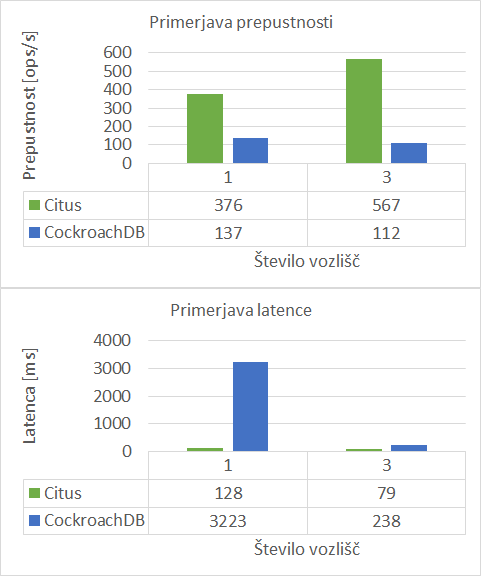
\includegraphics[width=0.7\textwidth]{resources/top-level-comparison.png}
\end{center}
\caption{Groba primerjava povprečne prepustnosti in latence med obema podatkovnima bazama na enem in treh vozliščih. Iz grafov je razvidno, da podatkovna baza CockroachDB dosega bistveno manjšo prepustnost, poleg tega pa ima večjo latenco.}
\label{img_ycsb_results_top_level_comparison}
\end{figure}

\newpage

\begin{figure}[H]
\begin{center}
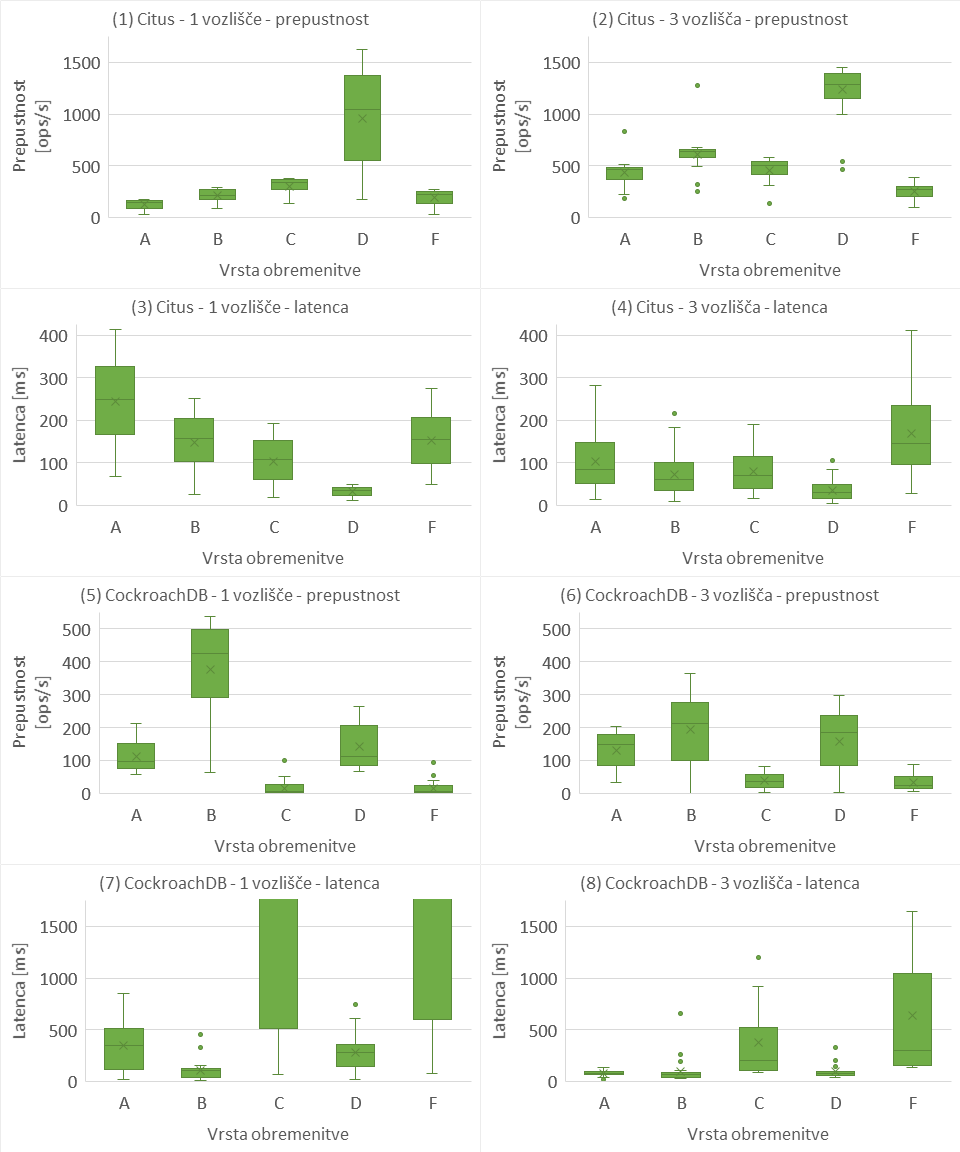
\includegraphics[width=1\textwidth]{resources/comparison-throughputnlatency-bnw.png}
\end{center}
\caption{Prikazuje primerjavo prepustnosti in latenc glede na vrsto obremenitve med podatkovno bazo Citus in CockroachDB. Graf (7) je zaradi lažje primerjave odrezan. Iz grafov je razvidno, da je podatkovna baza Citus v primerjavi s CockroachDB veliko bolj stabilna, kar se odraža v razponu med največjo in najmanjšo vrednostjo.}
\label{img_ycsb_results_bnw_comparison}
\end{figure}

\newpage

\begin{figure}[H]
\begin{center}
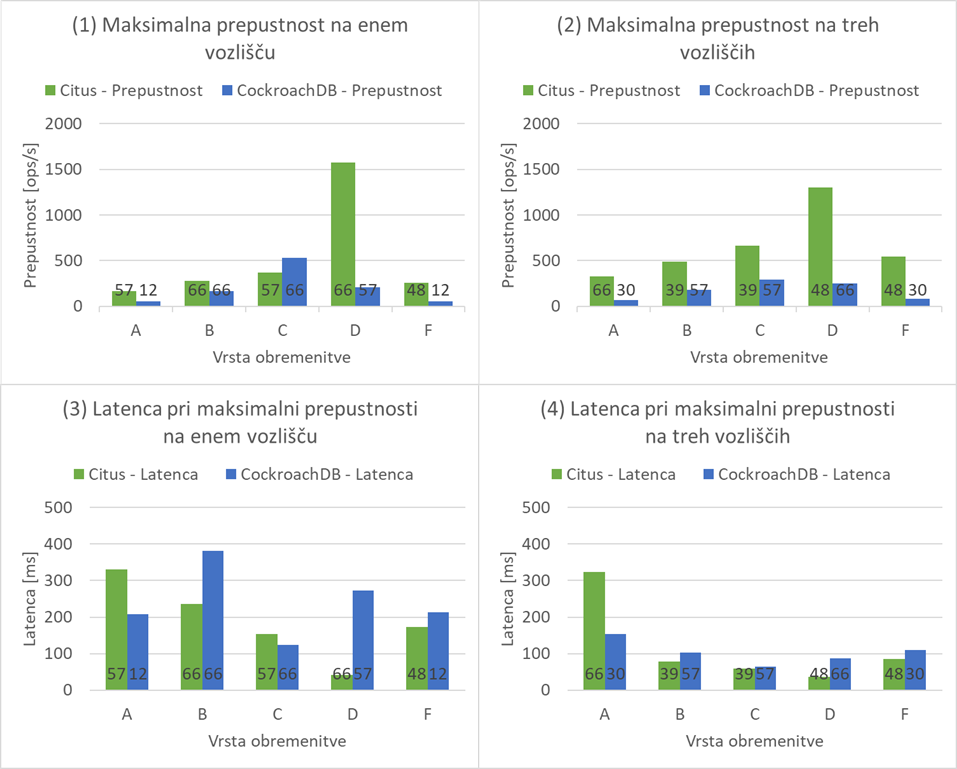
\includegraphics[width=1.0\textwidth]{resources/maxThroughput.png}
\end{center}
\caption{Prikazuje primerjavo prepustnosti in latence za vzorec z maksimalno prepustnostjo. Številke v spodnjem delu serije predstavljajo število sočasnih niti, pri katerih je bila dosežena maksimalna prepustnost. Iz grafov lahko razberemo, da se podatkovna baza CockroachDB z vidika sočasnih obremenitev skalira bolje kot Citus.}
\label{img_ycsb_results_max_throughput}
\end{figure}

\newpage

\section{Ugotovitve}
Zmogljivostna analiza je pokazala, da se podatkovna baza Citus pri večini obremenitev, katere smo testirali, odziva bistveno bolje kot podatkovna baza CockroachDB.

S slike \ref{img_ycsb_results_top_level_comparison} je razvidno, da CockroachDB v primerjavi s Citus dosega 2,7-krat manjšo prepustnost na enem vozlišču in kar 5-krat manjšo prepustnost na treh vozliščih. Pri primerjavi latence pa je CockroachDB v primerjavi s Citus na enem vozlišču dosegel približno 25,2-krat večjo latenco, na treh vozliščih pa samo še 3-krat večjo.

S slike \ref{img_ycsb_results_bnw_comparison} je razvidno, da je podatkovna baza CockroachDB v primerjavi s podatkovno bazo Citus manj stabilna. To se odraža na posameznih grafih, saj so rezultati meritev pri podatkovni bazi CockroachDB veliko bolj razpršeni.

Če primerjamo spremembe sočasnih niti, pri katerih sta bazi dosegali maksimalno prepustnost (slika \ref{img_ycsb_results_max_throughput}), opazimo naslednje. Podatkovna baza CockroachDB ob skaliranju na tri vozlišča lahko v povprečju obdela 5,4 več sočasnih niti, podatkovna baza Citus pa kar 10,8 manj.

\subsection{Hipoteza 1}
\textit{CockroachDB bo na enem vozlišču nekoliko počasnejši od PostgreSQL podatkovne baze.}

\ \\
Razlog za to hipotezo je, da je podatkovna baza PostgreSQL že dolgo na trgu \cite{Postgres-first-release} in je uporabljena na mnogih projektih. Zato je zmogljivostno bolje optimizirana, kakor CockroachDB. CockroachDB pa je na trgu od leta 2015. Prvo stabilno verzijo (1.0.0) so objavili maja 2017 \cite{CRDB-2017}, druga verzija (2.0.0) pa je bila objavljena aprila 2018. Vsaka verzija je dodala veliko novih funkcionalnosti.

Hipotezo smo potrdili, kar je razvidno tudi na sliki \ref{img_ycsb_results_top_level_comparison}. Podatkovna baza CockroachDB v primerjavi s PostgreSQL dosega približno 2,7-krat nižjo prepustnost.

Podobno zmogljivostno primerjavo so decembra 2017 izvedli na zasebni raziskovalni univerzi v Bruslju \cite{CRDB-2017}. Z orodjem YCSB (verzija 0.12.0) so primerjali obremenitve tipa A, B in C. Ugotovili so, da se podatkovna baza CockroachDB (verzija 1.1.3) v primerjavi s PostgreSQL (verzija 9.6.5) odziva približno 10-krat slabše, kakor PostgreSQL. V njihovem primeru so testno okolje postavili v Amazon oblaku, vsako bazo na treh vozliščih.

\subsection{Hipoteza 2}
\textit{CockroachDB bo zaradi linearne skalabilnosti na treh vozliščih skoraj 3-krat bolj zmogljiv.}

\ \\
Vsa vozlišča, povezana v CockroachDB gručo, so simetrična, kar pomeni, da vsa vozlišča opravljajo enake naloge. Ob predpostavki, da se uporabniki enakomerno razporedijo preko vseh vozlišč, ter da je obremenitev enakomerna, naj bi bila rast prepustnosti linearna \cite{CRDB-design}.

To hipotezo smo ovrgli. Meritve so pokazale, da podatkovna baza CockroachDB doseže celo slabšo prepustnost na treh vozliščih. To je razvidno iz slike \ref{img_ycsb_results_top_level_comparison}.

Razlog za tak rezultat naj bi bila primerjava med konfiguracijo na enem in treh vozliščih \cite{CRDB-YCSB-perf-analisis}. CockroachDB na treh vozliščih s privzetimi nastavitvami začne s postopkom replikacije podatkov. Privzeto je vsak podatek repliciran trikrat, enkrat na vsakem vozlišču. CockroachDB tako zagotavlja konsistenco in visoko razpoložljivost.

Rezultati neuradne TPC-C zmogljivostne analize, katero so izvedli v Co\-ckroachLabs, kažejo, da je CockroachDB linearno skalabilen \cite{CRDB-TPCC-perforamance-report}. Ob skali\-ranju iz 3 na 30 vozlišč ter ob sorazmernem povečanju obremenitve so dosegli tudi sorazmerno večjo prepustnost.

Prišli smo do ugotovitve, da je CockroachDB linearno skalabilna podatkovna baza (1), če je obremenitev enakomerno porazdeljena med vsa vozlišča in (2) faktor replikacije ob skaliranju ostane konstanten.

Na podlagi teh ugotovitev smo pripravili optimistično oceno rasti povprečne prepustnosti. Obe bazi se v idealnih pogojih in do neke mere skalirata linearno, kar je prikazano na sliki \ref{img_ycsb_results_scaling_throughptu_prediction}. Vendar pa se pri PostgreSQL konfiguraciji vsi odjemalci neposredno povezujejo na eno vozlišče (koordinatorja), ki je ozko grlo (točka A), saj bo ob večanju v neki točki prišlo do zasičenosti resursov \cite{Citus-add-coordinator}. V neki točki (točka B) pa bo CockroachDB presegel prepustnost podatkovne baze Citus.

\begin{figure}[H]
\begin{center}
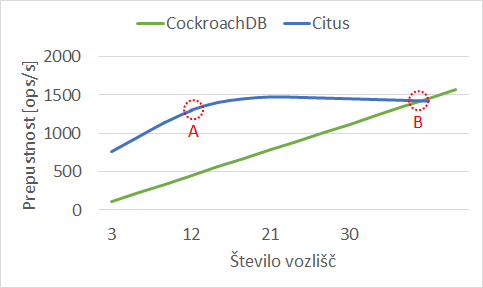
\includegraphics[width=0.7\textwidth]{resources/scaling-throughput-prediction-v2.png}
\end{center}
\caption{Optimistična ocena rasti povprečne prepustnosti. Pri podatkovni bazi Citus se v točki A linearna rast konča. V točki B pa ima CockroachDB že večjo prepustnost. Graf je le simboličen in ne predstavlja realnih meritev.}
\label{img_ycsb_results_scaling_throughptu_prediction}
\end{figure}


\chapter{Sklepne ugotovitve}

V diplomskem delu smo pregledali lastnosti  ter najpogosteje uporabljene mehanizme in pristope pri implementacijah novih arhitektur NewSQL podatkovnih baz. Opisali smo arhitekturo in lastnosti izbrane NewSQL podatkovne baze CockroachDB \cite{CRDB-home}. Podatkovno bazo CockroachDB smo kasneje praktično testirali. Izvedli smo primerjalno analizo zmogljivosti med podatkovno bazo CockroachDB in PostgreSQL \cite{postgres} (z nameščeno razširitvijo Citus \cite{citus}). Veliko časa smo vložili v postavitev testnega okolja in bili pozorni, da smo odpravili čim več spremenljivk, ki bi lahko vplivale na testne scenarije. Testno okolje je bilo sestavljeno iz štirih starejših računalnikov, ki so bili povezani preko gigabitnega omrežja, na njih pa je tekel Ubuntu Server \cite{ubuntu-server} in Docker \cite{docker}. Testno okolje smo v začetku nadzirali preko Telegraf agenta \cite{telegraf}, InfluxDB podatkovne baze za shranjevanje časovnih podatkov \cite{influxdb} in Grafane za vizualizacijo podatkov \cite{grafana}. Kljub trudu, ki smo ga vložili v postavitev testnega okolja, bi tega lahko še izboljšali. Za boljšo primerljivost zmogljivostnih metrik bi morala imeti vsa vozlišča enako strojno opremo, testirati pa bi moral še konfiguracije z več kot tremi vozlišči. Izvedbo testiranja smo avtomatizirali. Z orodjem YCSB \cite{brianfrankcooper/YCSB} smo izvajali različne zmogljivostne teste, rezultate pa shranjevali v CSV datoteko in jih kasneje analizirali.

Primerjalna analiza zmogljivosti je pokazala, da je podatkovna baza Cock\-roachDB kljub enostavnim obremenitvam, katere vrši orodje YCSB, v večini primerov bistveno slabša od PostgreSQL podatkovne baze. V povprečju je imela podatkovna baza Cock\-roachDB 3-krat večjo latenco in 5-krat manjšo prepustnost kakor podatkovna baza PostgreSQL na treh vozliščih.
% Poleg tega pa je z večanjem sočasnih povezav zmogljivost padala bistveno hitreje kot pri podatkovni bazi PostgreSQL.
Kljub slabšim rezultatom zmogljivostne analize se moramo zavedati, da je težko pošteno primerjati dve zelo različni podatkovni bazi. Podatkovna baza PostgreSQL je bistveno starejša in zato bolj stabilna ter optimizirana. CockroachDB pa je na trgu šele dobri dve leti in je trenutno še vedno bolj funkcionalno usmerjena. Za smiselno odločitev pri izbiri podatkovne baze moramo poleg zmogljivostnih metrik upoštevati tudi druge, kot so poizvedovalni jezik, podpora transakcijam, zrelost sistema, skupnost, zmogljivost, težavnost postavitve ter vzdrževanja, ostale lastnosti, specifične za vsako podatkovno bazo ...

Podatkovna baza CockroachDB ima močno in aktivno skupnost. Na spletu najdemo že kar nekaj vrednotenj drugih avtorjev, od raznih primerjalnih analiz \cite{kaur2017performance, Benchmarking-GCS-CRDB-NuoDB, CRDB-tpcc-vs-aurora, CRDB-2017}, do Jepsen testov konsistence in obnašanja sistema med napakami \cite{CRDB-jepsen, CRDB-jepsen-diy}.

Kljub temu, da je CockroachDB relativno nova podatkovna baza, jo podjeta že uporabljajo. Na primer podjetje Baidu \cite{crdb-baidu} uporablja CockroachDB pri dveh novih aplikacijah, ki sta predhodno uporabljale MySQL podatkovno bazo. Ti dve aplikaciji obsegata približno 2 TB podatkov in ustvarita približno 50 M zapisov na dan. Podjetje Kindred \cite{crdb-kindred} se ukvarja s spletnim igralništvom, z letom 2014 pa so začeli s prehodom na globalni trg. Imajo kompleksen ekosistem z več kot 200 mikrostoritvami. Ta arhitektura omogoča elastičnost, vendar pa mora biti skoraj v celoti avtonomna. CockroachLabs poizkuša s podjetji sodelovati, nekatera podjetja so tudi prispevala del funkcionalnosti. Podjetja, katera so se odločila za uporabo podatkovne baze CockroachDB, ciljajo globalni trg, poleg tega pa želijo poenostaviti postavitev in vzdrževanje, tako v oblaku, kakor tudi na svoji infrastrukturi.

Glede na znanje, katerega smo pridobili skozi diplomsko delo, menimo, da je podatkovna baza CockroachDB primerna za nove transakcijsko usmerjene (OLTP) aplikacije, katere zahtevajo konsistenco in visoko razpoložljivost, hkrati pa ciljajo hitrorastoč globalni trg ter za aplikacije, kjer je čas do trga zelo pomemben in kjer si ne moremo privoščiti velikih stroškov vzdrževanja. Pred odločitvijo moramo oceniti še podprto sintakso SQL jezika \cite{CRDB-sql-features} in morebitne ostale lastnosti \cite{CRDB-limitations}. Podatkovna baza CockroachDB trenutno ni primerna za scenarije, ki zahtevajo kompleksne stične operacije, nizko latenco in analitično usmerjene aplikacije (OLAP) \cite{CRDB-FAQ}.

V prihodnje bi bilo zanimivo raziskati in primerjati še zelo podobno in prav tako odprtokodno podatkovno bazo TiDB \cite{PingCAP-home}. TiDB je trenutno še zelo mlad produkt, z verzijo 1.0.0, ki je izšla sredi oktobra 2017, in verzijo 2.0.0 iz aprila 2018. TiDB prav tako idejno temelji na podatkovni bazi Google Spanner in se v nekaterih arhitekturnih lastnostih zelo ujema s podatkovno bazo CockroachDB. Najbolj očitna razlika je, da je arhitektura ločena na tri večje komponente, poleg tega za sinhronizacijo ure uporablja drugačen pristop. Razvijalci podatkovne baze TiDB obljubljajo, da je podatkovna baza primerna za hibridne transakcijske in analitične obremenitve.

Zanimivo bi bilo tudi razširiti zmogljivostno primerjalno analizo, izvedeno v tem diplomskem delu. Porazdeljene podatkovne baze, kot je CockroachDB, so primerne za okolja z vsaj tremi vozlišči. Zanimivo bi bilo ugotoviti, kaj se dogaja, ko v gručo povežemo še več vozlišč. Poleg osnovnih YCSB obremenitev bi bilo zanimivo preveriti še druge, kot sta TPC-C in TPC-H.


\newpage %dodaj po potrebi, da bo številka strani za Literaturo v Kazalu pravilna!
\ \\
\clearpage
\addcontentsline{toc}{chapter}{Literatura}
\bibliographystyle{plain}
\bibliography{bibliography}


\end{document}

